\documentclass[aspectratio=43]{beamer}
\usepackage[czech]{babel}
\usepackage[utf8]{inputenc}
\usepackage[T1]{fontenc}
\usepackage{graphicx}
\usepackage{xcolor}
\usepackage{multirow}
\usepackage{tikz}

% Definice barev SPŠE
\definecolor{spseBurgundy}{RGB}{142, 85, 85}  % Upravená burgundy podle obrázku

% Odstranění navigačních symbolů
\setbeamertemplate{navigation symbols}{}

% Nastavení vzhledu
\useinnertheme{default}
\useoutertheme{default}

% Úprava pozadí a barev
\setbeamercolor{background canvas}{bg=white}
\setbeamercolor{frametitle}{fg=white,bg=spseBurgundy}
\setbeamercolor{title}{fg=black,bg=white}
\setbeamercolor{itemize item}{fg=spseBurgundy}
\setbeamercolor{itemize subitem}{fg=spseBurgundy}

% Nastavení rámečku titulu
\setbeamertemplate{frametitle}{
  \vspace*{-0.1cm}
  \begin{beamercolorbox}[wd=\paperwidth,ht=1cm,dp=0.2cm]{frametitle}
    \vspace*{0.1cm}\hspace*{1cm}\insertframetitle
  \end{beamercolorbox}
}

% Patička
\setbeamertemplate{footline}{%
   \begin{beamercolorbox}[wd=\paperwidth,ht=1cm,dp=0.2cm,left]{structure}
    \hspace*{0.5cm}
\includegraphics[height=0.6cm]{logo.png}%
    \hfill\hfill{\color{black}\insertshortsubtitle}\hfill%
    \hfill\hfill{\color{black}\insertframenumber/\inserttotalframenumber}\hspace*{0.5cm}%
  \end{beamercolorbox}
}

% Nastavení odrážek
\setbeamertemplate{itemize item}{\small\raise0.5pt\hbox{\donotcoloroutermaths$\blacksquare$}}
\setbeamertemplate{itemize subitem}{\small\raise0.5pt\hbox{\donotcoloroutermaths$\blacksquare$}}

\title{SBĚRNICE}
\subtitle{SBĚRNICE}
\author{Bc. David Zimniok}
\date{}

\begin{document}

% Titulní strana - speciální uspořádání
\begin{frame}[plain]
	\vspace*{-0.5cm}
	\begin{beamercolorbox}[wd=\paperwidth,ht=2cm,dp=0ex]{frametitle}
		\hspace*{0.5cm}
\includegraphics[height=1.4cm]{logo_w.png}
	\end{beamercolorbox}
	\vspace{1cm}
	\begin{flushright}
		{\textbf{\Large\inserttitle\par}}
		\vspace{0.1cm}
		{\large HARDWARE 4. ročníky \par}
        {\large verze 01/25 \par}
		\vspace{1.5cm}
		{\scriptsize\insertauthor\par}
		\vspace{0.1cm}
		{\scriptsize david.zimniok@spsehavirov.cz}
	\end{flushright}
	\vspace*{0.5cm}
	\hspace*{-0.4cm}
\includegraphics[height=1cm]{logo.png}
\end{frame}

\begin{frame}{}
	 
	\begin{center}
		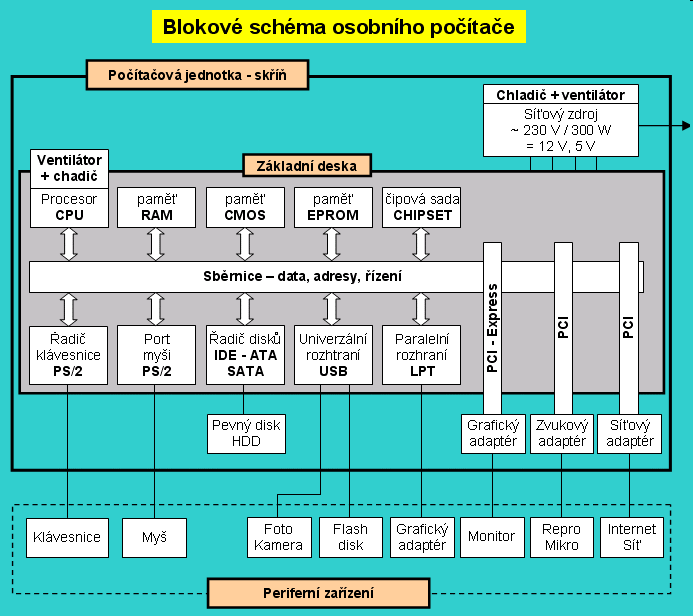
\includegraphics[width=0.9\linewidth]{extrahovane_obrazky/img_1_page1_0.png}
	\end{center}
	
\end{frame}

\section{Sběrnice}
\begin{frame}{Sběrnice}
	\begin{itemize}
		\item soustava logických prvků, vodičů, typů konektorů (tzv. rozhraní sběrnice) spojujících jednotlivé části počítače a sloužících k vzájemné výměně dat mezi nimi (reálná implementace sběrnice)
		\item soustava pravidel a definic, popisující konstrukční, elektrické a funkční parametry sběrnice (tzn. log. úrovně, taktovací frekvence, šířka sběrnice, s tím související rychlost a propustnost sběrnice),  umožňující bezchybně navrhnout bloky počítačetak, aby byly schopné po sběrnici komunikovat pro různé výrobce (specifikace sběrnice, kterou vydává nějaká organizace (JEDEC, Organizace PCI-SIG…)).
		      různých zařízení
	\end{itemize}
\end{frame}

\begin{frame}{Paralelní sběrnice}
	\begin{itemize}
		\item Datové (D0 – D15, D31 - D63) - podle datové šířky sběrnice
		\item Adresní (A0 – A15, A31) - podle možného adresního prostoru sběrnice
		\item Řídící (Clk, WE, CE, OE, MR, MW, I/OR, I/OW, BE, OE) -podle typu sběrnice
	\end{itemize}
		
		
		
	\begin{center}
		
		\resizebox{0.95\textwidth}{!}{
			\tikzset{every picture/.style={line width=0.75pt}} %set default line width to 0.75pt        
			
			\begin{tikzpicture}[x=0.75pt,y=0.75pt,yscale=-1,xscale=1]
				%uncomment if require: \path (0,300); %set diagram left start at 0, and has height of 300
				
				%Shape: Rectangle [id:dp5235078985659226] 
				\draw  [color={rgb, 255:red, 144; green, 19; blue, 254 }  ,draw opacity=1 ][fill={rgb, 255:red, 144; green, 19; blue, 254 }  ,fill opacity=1 ] (157.75,110.5) -- (571,110.5) -- (571,120) -- (157.75,120) -- cycle ;
				%Shape: Rectangle [id:dp6628524816745138] 
				\draw  [color={rgb, 255:red, 126; green, 211; blue, 33 }  ,draw opacity=1 ][fill={rgb, 255:red, 126; green, 211; blue, 33 }  ,fill opacity=1 ] (137,131.5) -- (571,131.5) -- (571,141) -- (137,141) -- cycle ;
				%Shape: Rectangle [id:dp5916183481599812] 
				\draw  [line width=1.5]  (106,21) -- (176,21) -- (176,61) -- (106,61) -- cycle ;
				
				%Shape: Rectangle [id:dp12637419466013822] 
				\draw  [line width=1.5]  (199,21) -- (276.5,21) -- (276.5,61) -- (199,61) -- cycle ;
				
				%Shape: Rectangle [id:dp9601745906204652] 
				\draw  [line width=1.5]  (400,21) -- (470,21) -- (470,61) -- (400,61) -- cycle ;
				
				%Shape: Rectangle [id:dp21976864156620513] 
				\draw  [line width=1.5]  (493.5,21) -- (563.5,21) -- (563.5,61) -- (493.5,61) -- cycle ;
				
				%Shape: Rectangle [id:dp5761294473680548] 
				\draw  [line width=1.5]  (299.5,21) -- (377,21) -- (377,61) -- (299.5,61) -- cycle ;
				
				%Up Arrow [id:dp7777757872817223] 
				\draw  [color={rgb, 255:red, 245; green, 166; blue, 35 }  ,draw opacity=1 ][fill={rgb, 255:red, 245; green, 166; blue, 35 }  ,fill opacity=1 ] (112.25,85.4) -- (120.25,63) -- (128.25,85.4) -- (124.25,85.4) -- (124.25,119) -- (116.25,119) -- (116.25,85.4) -- cycle ;
				%Up Arrow [id:dp19684936113056706] 
				\draw  [color={rgb, 255:red, 126; green, 211; blue, 33 }  ,draw opacity=1 ][fill={rgb, 255:red, 126; green, 211; blue, 33 }  ,fill opacity=1 ] (133,84.9) -- (141,62.5) -- (149,84.9) -- (145,84.9) -- (145,118.5) -- (137,118.5) -- (137,84.9) -- cycle ;
				%Up Arrow [id:dp012977859680316839] 
				\draw  [color={rgb, 255:red, 144; green, 19; blue, 254 }  ,draw opacity=1 ][fill={rgb, 255:red, 144; green, 19; blue, 254 }  ,fill opacity=1 ] (153.75,85.17) -- (161.75,62) -- (169.75,85.17) -- (165.75,85.17) -- (165.75,119.93) -- (157.75,119.93) -- (157.75,85.17) -- cycle ;
				%Shape: Rectangle [id:dp6856178914473671] 
				\draw  [color={rgb, 255:red, 245; green, 166; blue, 35 }  ,draw opacity=1 ][fill={rgb, 255:red, 245; green, 166; blue, 35 }  ,fill opacity=1 ] (116.25,119) -- (124.25,119) -- (124.25,159.83) -- (116.25,159.83) -- cycle ;
				%Shape: Rectangle [id:dp39386454661091075] 
				\draw  [color={rgb, 255:red, 126; green, 211; blue, 33 }  ,draw opacity=1 ][fill={rgb, 255:red, 126; green, 211; blue, 33 }  ,fill opacity=1 ] (137,118.5) -- (145,118.5) -- (145,141) -- (137,141) -- cycle ;
				%Up Arrow [id:dp741965115038404] 
				\draw  [color={rgb, 255:red, 245; green, 166; blue, 35 }  ,draw opacity=1 ][fill={rgb, 255:red, 245; green, 166; blue, 35 }  ,fill opacity=1 ] (499.75,85.4) -- (507.75,63) -- (515.75,85.4) -- (511.75,85.4) -- (511.75,119) -- (503.75,119) -- (503.75,85.4) -- cycle ;
				%Up Arrow [id:dp12519780116903523] 
				\draw  [color={rgb, 255:red, 126; green, 211; blue, 33 }  ,draw opacity=1 ][fill={rgb, 255:red, 126; green, 211; blue, 33 }  ,fill opacity=1 ] (520.5,84.9) -- (528.5,62.5) -- (536.5,84.9) -- (532.5,84.9) -- (532.5,118.5) -- (524.5,118.5) -- (524.5,84.9) -- cycle ;
				%Up Arrow [id:dp5581921957847968] 
				\draw  [color={rgb, 255:red, 144; green, 19; blue, 254 }  ,draw opacity=1 ][fill={rgb, 255:red, 144; green, 19; blue, 254 }  ,fill opacity=1 ] (541.25,84.97) -- (549.25,62) -- (557.25,84.97) -- (553.25,84.97) -- (553.25,119.43) -- (545.25,119.43) -- (545.25,84.97) -- cycle ;
				%Shape: Rectangle [id:dp9638717795221039] 
				\draw  [color={rgb, 255:red, 245; green, 166; blue, 35 }  ,draw opacity=1 ][fill={rgb, 255:red, 245; green, 166; blue, 35 }  ,fill opacity=1 ] (503.75,119) -- (511.75,119) -- (511.75,159.83) -- (503.75,159.83) -- cycle ;
				%Shape: Rectangle [id:dp8865388625935862] 
				\draw  [color={rgb, 255:red, 126; green, 211; blue, 33 }  ,draw opacity=1 ][fill={rgb, 255:red, 126; green, 211; blue, 33 }  ,fill opacity=1 ] (524.5,118.5) -- (532.5,118.5) -- (532.5,141) -- (524.5,141) -- cycle ;
				%Up Arrow [id:dp088025773880412] 
				\draw  [color={rgb, 255:red, 245; green, 166; blue, 35 }  ,draw opacity=1 ][fill={rgb, 255:red, 245; green, 166; blue, 35 }  ,fill opacity=1 ] (209.13,85.4) -- (217.13,63) -- (225.13,85.4) -- (221.13,85.4) -- (221.13,119) -- (213.13,119) -- (213.13,85.4) -- cycle ;
				%Up Arrow [id:dp08403873794261796] 
				\draw  [color={rgb, 255:red, 126; green, 211; blue, 33 }  ,draw opacity=1 ][fill={rgb, 255:red, 126; green, 211; blue, 33 }  ,fill opacity=1 ] (229.88,84.9) -- (237.88,62.5) -- (245.88,84.9) -- (241.88,84.9) -- (241.88,118.5) -- (233.88,118.5) -- (233.88,84.9) -- cycle ;
				%Up Arrow [id:dp33590036904325815] 
				\draw  [color={rgb, 255:red, 144; green, 19; blue, 254 }  ,draw opacity=1 ][fill={rgb, 255:red, 144; green, 19; blue, 254 }  ,fill opacity=1 ] (250.63,85.17) -- (258.63,62) -- (266.63,85.17) -- (262.63,85.17) -- (262.63,119.93) -- (254.63,119.93) -- (254.63,85.17) -- cycle ;
				%Shape: Rectangle [id:dp9148176696614055] 
				\draw  [color={rgb, 255:red, 245; green, 166; blue, 35 }  ,draw opacity=1 ][fill={rgb, 255:red, 245; green, 166; blue, 35 }  ,fill opacity=1 ] (213.13,119) -- (221.13,119) -- (221.13,159.83) -- (213.13,159.83) -- cycle ;
				%Shape: Rectangle [id:dp06740495718701067] 
				\draw  [color={rgb, 255:red, 126; green, 211; blue, 33 }  ,draw opacity=1 ][fill={rgb, 255:red, 126; green, 211; blue, 33 }  ,fill opacity=1 ] (233.88,118.5) -- (241.88,118.5) -- (241.88,141) -- (233.88,141) -- cycle ;
				%Up Arrow [id:dp3671011147263876] 
				\draw  [color={rgb, 255:red, 245; green, 166; blue, 35 }  ,draw opacity=1 ][fill={rgb, 255:red, 245; green, 166; blue, 35 }  ,fill opacity=1 ] (306.01,85.4) -- (314.01,63) -- (322.01,85.4) -- (318.01,85.4) -- (318.01,119) -- (310.01,119) -- (310.01,85.4) -- cycle ;
				%Up Arrow [id:dp20076469071022673] 
				\draw  [color={rgb, 255:red, 126; green, 211; blue, 33 }  ,draw opacity=1 ][fill={rgb, 255:red, 126; green, 211; blue, 33 }  ,fill opacity=1 ] (326.76,84.9) -- (334.76,62.5) -- (342.76,84.9) -- (338.76,84.9) -- (338.76,118.5) -- (330.76,118.5) -- (330.76,84.9) -- cycle ;
				%Up Arrow [id:dp7493885475396296] 
				\draw  [color={rgb, 255:red, 144; green, 19; blue, 254 }  ,draw opacity=1 ][fill={rgb, 255:red, 144; green, 19; blue, 254 }  ,fill opacity=1 ] (347.51,85.17) -- (355.51,62) -- (363.51,85.17) -- (359.51,85.17) -- (359.51,119.93) -- (351.51,119.93) -- (351.51,85.17) -- cycle ;
				%Shape: Rectangle [id:dp034275129350830436] 
				\draw  [color={rgb, 255:red, 245; green, 166; blue, 35 }  ,draw opacity=1 ][fill={rgb, 255:red, 245; green, 166; blue, 35 }  ,fill opacity=1 ] (310.01,119) -- (318.01,119) -- (318.01,159.83) -- (310.01,159.83) -- cycle ;
				%Shape: Rectangle [id:dp5219512103240798] 
				\draw  [color={rgb, 255:red, 126; green, 211; blue, 33 }  ,draw opacity=1 ][fill={rgb, 255:red, 126; green, 211; blue, 33 }  ,fill opacity=1 ] (330.76,118.5) -- (338.76,118.5) -- (338.76,141) -- (330.76,141) -- cycle ;
				%Up Arrow [id:dp8614302264576735] 
				\draw  [color={rgb, 255:red, 245; green, 166; blue, 35 }  ,draw opacity=1 ][fill={rgb, 255:red, 245; green, 166; blue, 35 }  ,fill opacity=1 ] (402.89,85.4) -- (410.89,63) -- (418.89,85.4) -- (414.89,85.4) -- (414.89,119) -- (406.89,119) -- (406.89,85.4) -- cycle ;
				%Up Arrow [id:dp8783705565550148] 
				\draw  [color={rgb, 255:red, 126; green, 211; blue, 33 }  ,draw opacity=1 ][fill={rgb, 255:red, 126; green, 211; blue, 33 }  ,fill opacity=1 ] (423.64,84.9) -- (431.64,62.5) -- (439.64,84.9) -- (435.64,84.9) -- (435.64,118.5) -- (427.64,118.5) -- (427.64,84.9) -- cycle ;
				%Up Arrow [id:dp53838488416421] 
				\draw  [color={rgb, 255:red, 144; green, 19; blue, 254 }  ,draw opacity=1 ][fill={rgb, 255:red, 144; green, 19; blue, 254 }  ,fill opacity=1 ] (444.39,84.97) -- (452.39,62) -- (460.39,84.97) -- (456.39,84.97) -- (456.39,119.43) -- (448.39,119.43) -- (448.39,84.97) -- cycle ;
				%Shape: Rectangle [id:dp8145183791944111] 
				\draw  [color={rgb, 255:red, 245; green, 166; blue, 35 }  ,draw opacity=1 ][fill={rgb, 255:red, 245; green, 166; blue, 35 }  ,fill opacity=1 ] (406.89,119) -- (414.89,119) -- (414.89,159.83) -- (406.89,159.83) -- cycle ;
				%Shape: Rectangle [id:dp15652984968228334] 
				\draw  [color={rgb, 255:red, 126; green, 211; blue, 33 }  ,draw opacity=1 ][fill={rgb, 255:red, 126; green, 211; blue, 33 }  ,fill opacity=1 ] (427.64,118.5) -- (435.64,118.5) -- (435.64,141) -- (427.64,141) -- cycle ;
				%Shape: Rectangle [id:dp7017822899342713] 
				\draw  [color={rgb, 255:red, 245; green, 166; blue, 35 }  ,draw opacity=1 ][fill={rgb, 255:red, 245; green, 166; blue, 35 }  ,fill opacity=1 ] (116.25,150.5) -- (570.5,150.5) -- (570.5,159.83) -- (116.25,159.83) -- cycle ;
				
				
				% Text Node
				\draw (116.25,149.5) node [anchor=north west][inner sep=0.75pt]  [font=\tiny] [align=left] {\textbf{ADDRESS LINES}};
				% Text Node
				\draw (137,130.5) node [anchor=north west][inner sep=0.75pt]  [font=\tiny] [align=left] {\textbf{CONTROL LINES}};
				% Text Node
				\draw (157.75,109.5) node [anchor=north west][inner sep=0.75pt]  [font=\tiny,color={rgb, 255:red, 255; green, 255; blue, 255 }  ,opacity=1 ] [align=left] {\textbf{DATA LINES}};
				% Text Node
				\draw (472.5,27) node [anchor=north west][inner sep=0.75pt]   [align=left] {\textbf{...}};
				% Text Node
				\draw (279,27) node [anchor=north west][inner sep=0.75pt]   [align=left] {\textbf{...}};
				% Text Node
				\draw (301.75,29.5) node [anchor=north west][inner sep=0.75pt]   [align=left] {\textbf{MEMORY}};
				% Text Node
				\draw (515.5,29.5) node [anchor=north west][inner sep=0.75pt]   [align=left] {\textbf{I/O}};
				% Text Node
				\draw (422,29.5) node [anchor=north west][inner sep=0.75pt]   [align=left] {\textbf{I/O}};
				% Text Node
				\draw (201.25,29.5) node [anchor=north west][inner sep=0.75pt]   [align=left] {\textbf{MEMORY}};
				% Text Node
				\draw (122,29.5) node [anchor=north west][inner sep=0.75pt]   [align=left] {\textbf{CPU}};
				
				
			\end{tikzpicture}
		}
	\end{center}
		
\end{frame}

\begin{frame}{Sběrnice - rozdělení}
	\begin{table}[]
		\begin{tabular}{|c|c|}
			\hline
			\textbf{paralelní}   & \textbf{sériové}     \\
			PCI, PCI-X            & PCI Express, USB       \\ \hline
			\textbf{interní}     & \textbf{externí}      \\
			ISA, PCI, PCI express & USB, FireWare          \\ \hline
			\textbf{lokální}    & \textbf{univerzální} \\
			VL–Bus              & PCI                    \\ \hline
		\end{tabular}
	\end{table}
\end{frame}


\begin{frame}{Vývoj sběrnic PC}
	
	\begin{columns}
		\column{0.39\textwidth}
        \begin{figure}[ht]
            \centering
            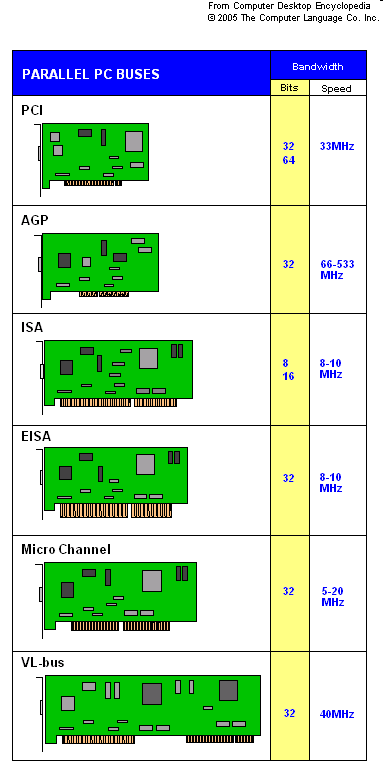
\includegraphics[width=0.85\linewidth]{extrahovane_obrazky/img_1_page6_0.png}
        \end{figure}
		\column{0.59\textwidth}
		\begin{itemize}
			\item ISA (Industry Standard Architecture)
			\item 1981 – 8-bitová verze
			\item 1984 – 16-bitová verze (AT bus)
			\item Adresa 24 bitů, Data 16 bitů
			\item Frekvence 4.77, 8, 8.33, 10, 12 a 14 MHz
		\end{itemize}
        \begin{minipage}{\textwidth}
            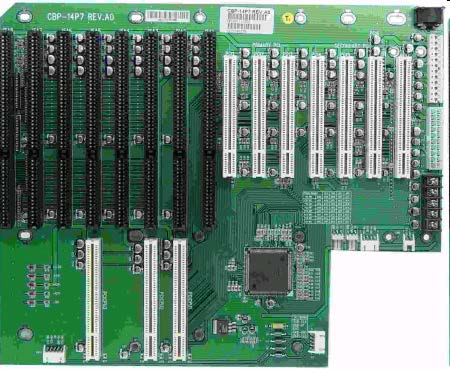
\includegraphics[width=0.48\textwidth]{extrahovane_obrazky/img_1_page6_15.jpeg}
            \hfill
            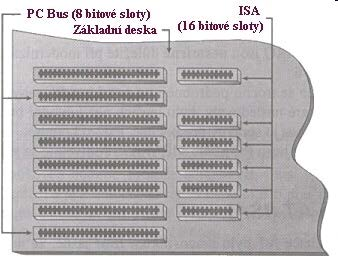
\includegraphics[width=0.48\textwidth]{extrahovane_obrazky/img_1_page6_16.jpeg}
        \end{minipage}
	\end{columns}
	
\end{frame}


\begin{frame}{Vývoj sběrnic PC}
	
	\begin{columns}
		\column{0.39\textwidth}
		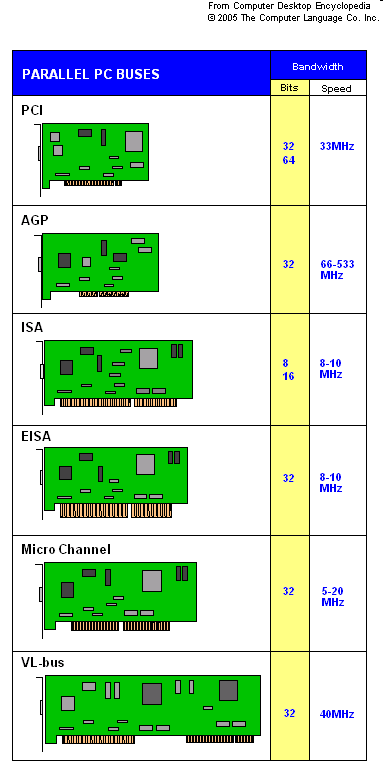
\includegraphics[width=0.85\linewidth]{extrahovane_obrazky/img_1_page6_0.png}
		\column{0.59\textwidth}
		\begin{itemize}
			\item MCA (Micro Channel Architecture)
			\item byla vyvinuta firmou IBM pro počítače řady PS/2
			\item není zpětně kompatibilní se sběrnicí ISA
			\item maximální frekvence 10 MHz
			\item šířka přenosu dat je 16, resp. 32 bitů
		\end{itemize}
        \vspace{0.5}
		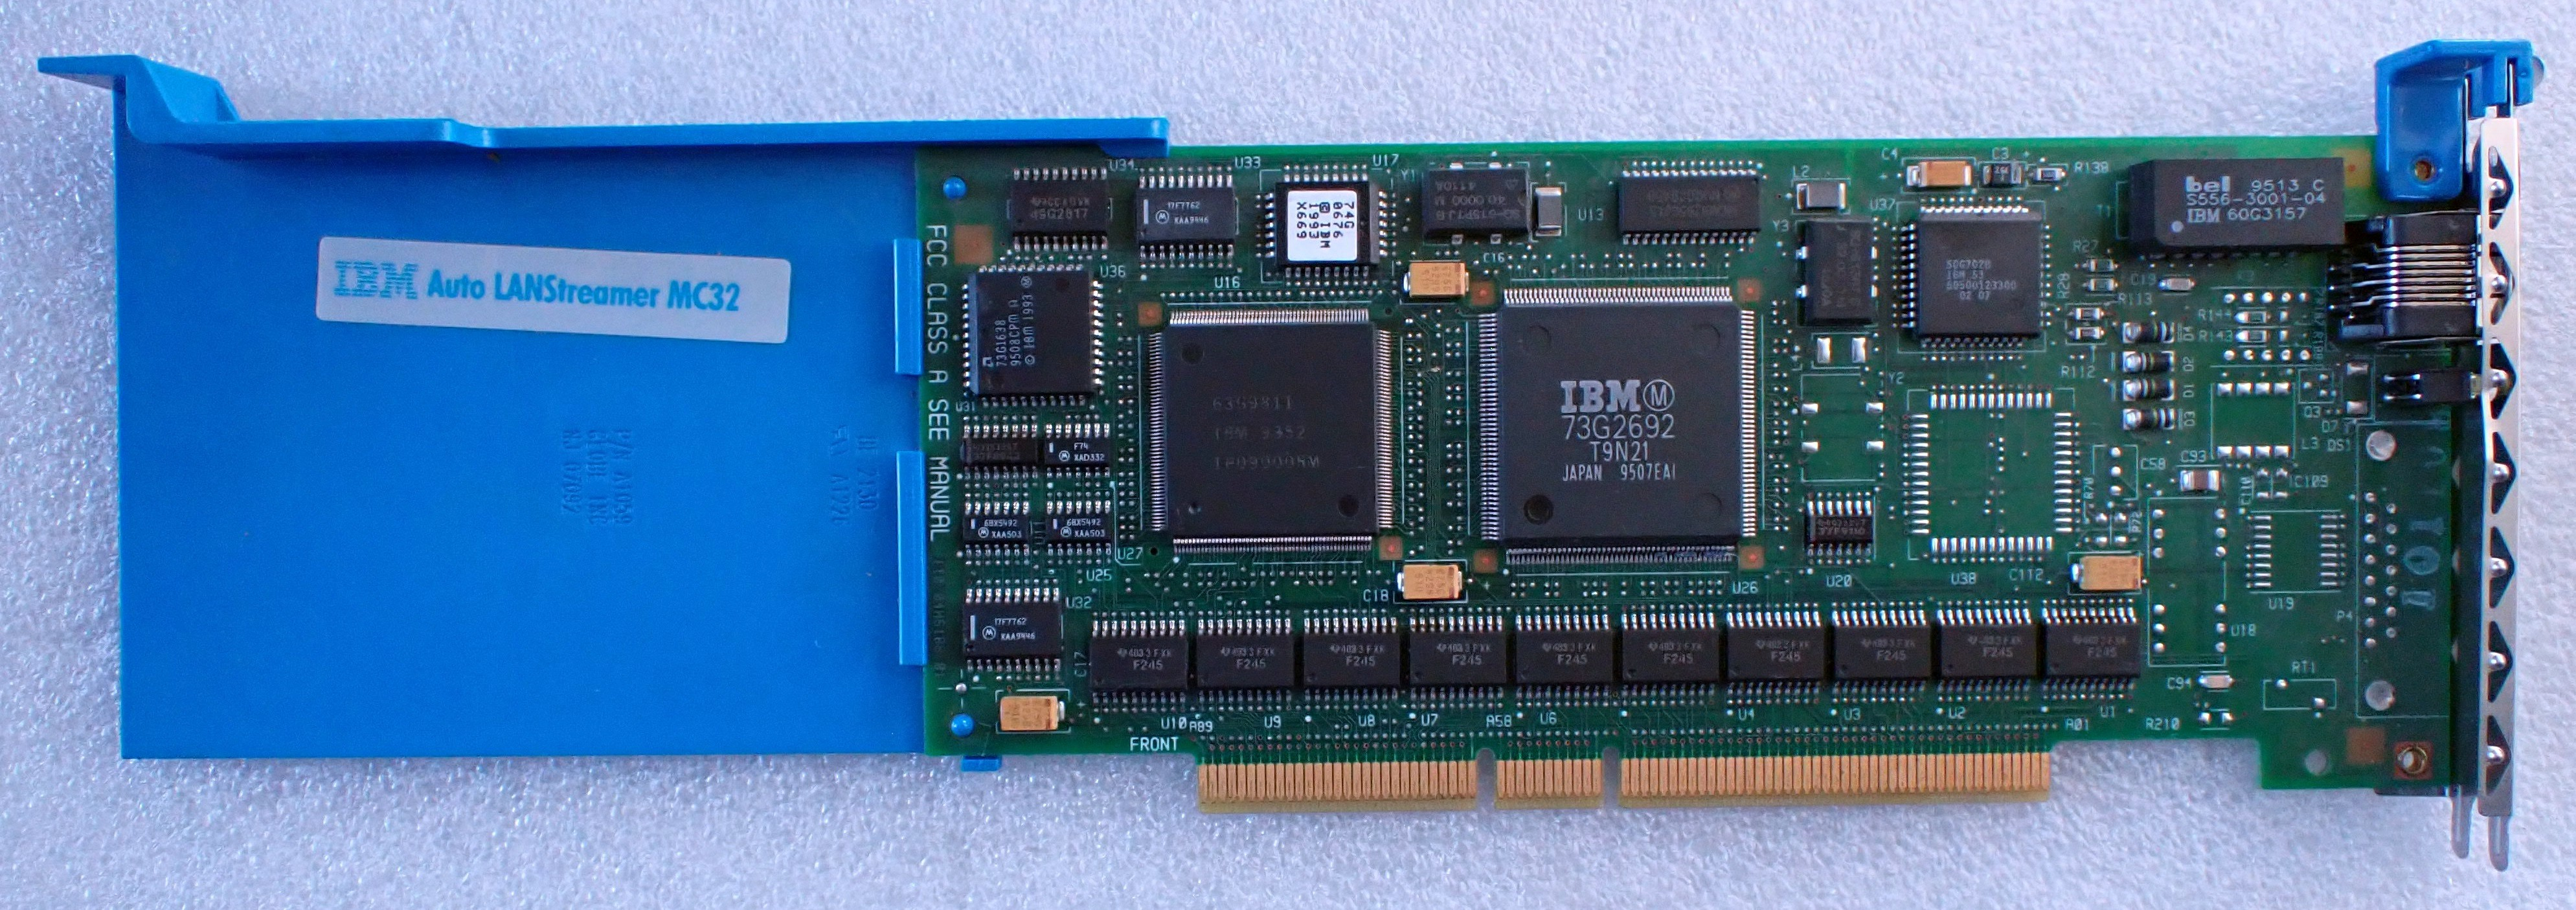
\includegraphics[width=1\linewidth]{extrahovane_obrazky/mca.jpeg}
	\end{columns}
	
\end{frame}


\begin{frame}{Vývoj sběrnic PC}
	\begin{columns}
		\column{0.39\textwidth}
		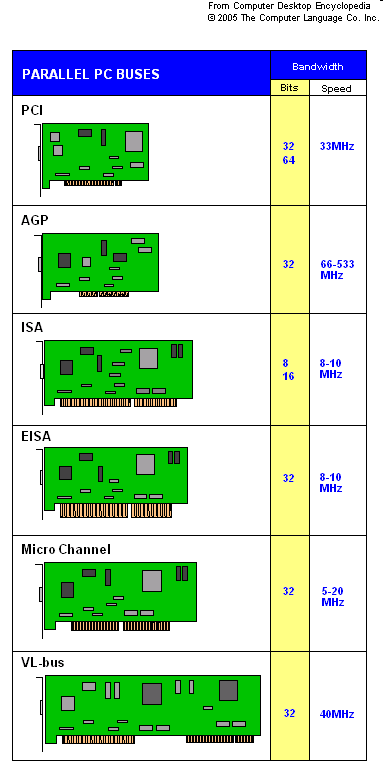
\includegraphics[width=0.85\linewidth]{extrahovane_obrazky/img_1_page6_0.png}
		\column{0.59\textwidth}
		\begin{itemize}
			\item EISA (Extended Industry Standard Architecture)
			\item byla vyrobena 9 firmami jako odpověď na sběrnici MCA
			\item kompatibilní se sběrnicí ISA
			\item šířka přenosu dat je 32 bitů
			\item frekvence 8 MHz (z důvodů kompatibility s ISA)
		\end{itemize}
		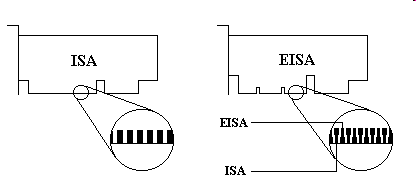
\includegraphics[width=1\linewidth]{extrahovane_obrazky/img_1_page8_3.png}
	\end{columns}
	
\end{frame}


\begin{frame}{Vývoj sběrnic PC}
	
	\begin{columns}
		\column{0.39\textwidth}
		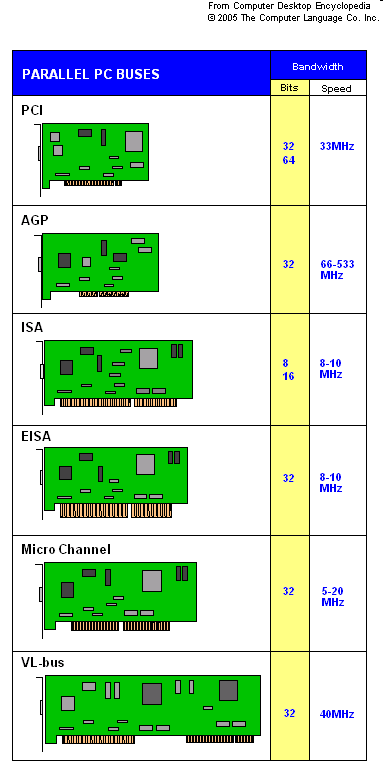
\includegraphics[width=0.85\linewidth]{extrahovane_obrazky/img_1_page6_0.png}
		\column{0.59\textwidth}
		\begin{itemize}
			\item VESA Local Bus
			\item lokální sběrnice
			\item jako rychlejší doplněk k výkonnostně nedostatečné sběrnici ISA.
		\end{itemize}
        \vspace{0.5}
		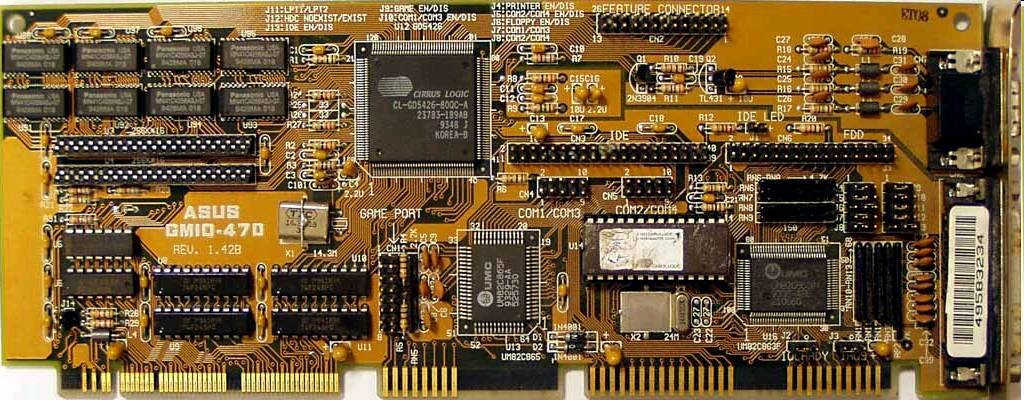
\includegraphics[width=1\linewidth]{extrahovane_obrazky/img_1_page9_7.jpeg}
	\end{columns}
	
\end{frame}

\section{PCI}
\begin{frame}{Základní podoba architektury PC se sběrnicí PCI}
	\begin{itemize}
        \item Rok 1995
        \item sběrnice podporovala 66 MHz protokol
        \item volitelná šířka přenosu 32/64 bitů
        \item podpora Plug and Play, procesorově nezávislá
        \item Původní model architektury PC se sběrnicí PCI: kooperace PCI se systémovou sběrnicíprocesoru (FSB – Front Side Bus) oddělení zajišťoval PCI most, což byl adaptér sběrnice PCI na rozhraní FSB.
        \item Prostředky pro obsluhu sběrnice PCI rozděleny do dvou pevně definovaných částí: northbridge (spravoval komunikaci s procesorem a pamětí) a southbridge (pomalé periferie).
    \end{itemize}
	
\end{frame}

\begin{frame}{Základní podoba architektury PC se sběrnicí PCI}
    \begin{center}
        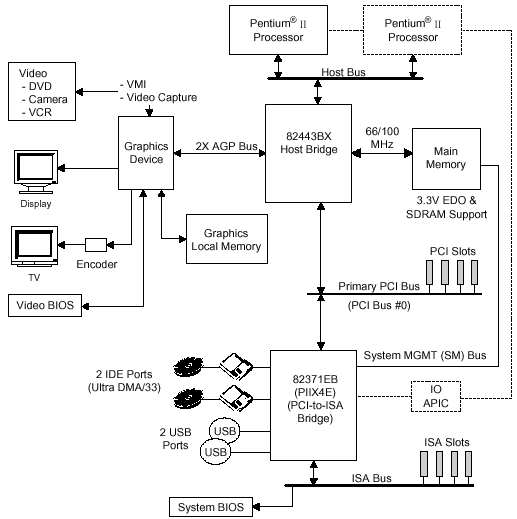
\includegraphics[width=0.7\linewidth]{extrahovane_obrazky/img_1_page10_0.png}
    \end{center}
\end{frame}



\begin{frame}{Sběrnice  PCI}
	\begin{itemize}
		\item PCI je paralelní a polo-duplexní - všechny vodiče slouží pro přenos dat oběma směry, ovšem nikoli oběma směry zároveň
		\item Na rozdíl třeba od sběrnice ISA nemá PCI adresní část oddělenou od části datové - charakteristický počet vodičů (32 nebo 64) slouží pro přenos dat i adres, adresa se posílá na začátku každé transakce.
	\end{itemize}
	
\end{frame}


\begin{frame}{Varianty sběrnic PCI}
	\begin{columns}
		\column{0.49\textwidth}
        \begin{center}
            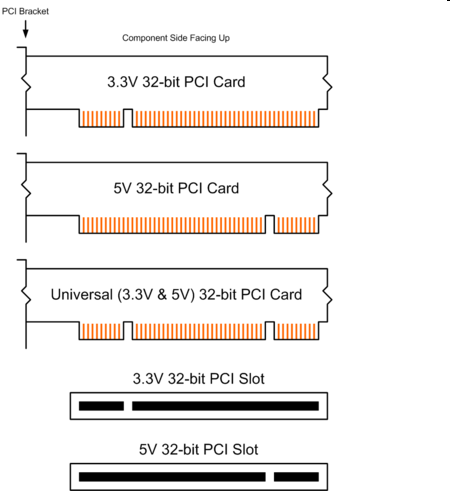
\includegraphics[width=1\linewidth]{extrahovane_obrazky/img_1_page12_1.png}
        \end{center}
		\column{0.49\textwidth}
        \begin{center}
            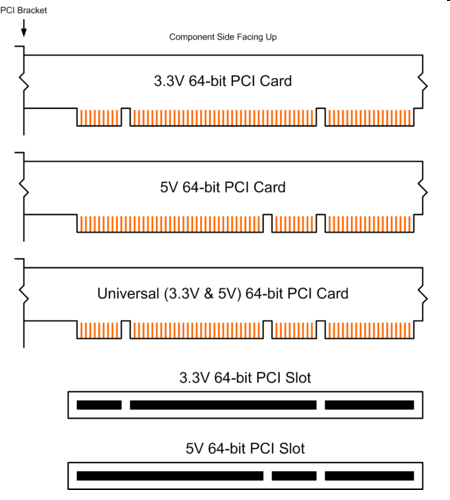
\includegraphics[width=1\linewidth]{extrahovane_obrazky/img_1_page12_2.png}
        \end{center}
	\end{columns}
	 
\end{frame}

\begin{frame}{Verze PCI - X}
	\begin{itemize}
		\item PCI-X podporuje frekvenci až 533 MHz (oproti max. 66 MHz u PCI)
		\item 32bitové i 64bitové šířky přenosu
		\item Zpětná kompatibilita – PCI-X podporuje starší PCI karty, ale ty pak běží na nižší rychlosti.
		\item Byla využívána pro síťové adaptéry, RAID řadiče a další výkonné komponenty.
		\item Pokud do PCI-X slotu připojíte pomalejší kartu PCI, může zpomalit celou sběrnici.
	\end{itemize}
	 
	\begin{center}
		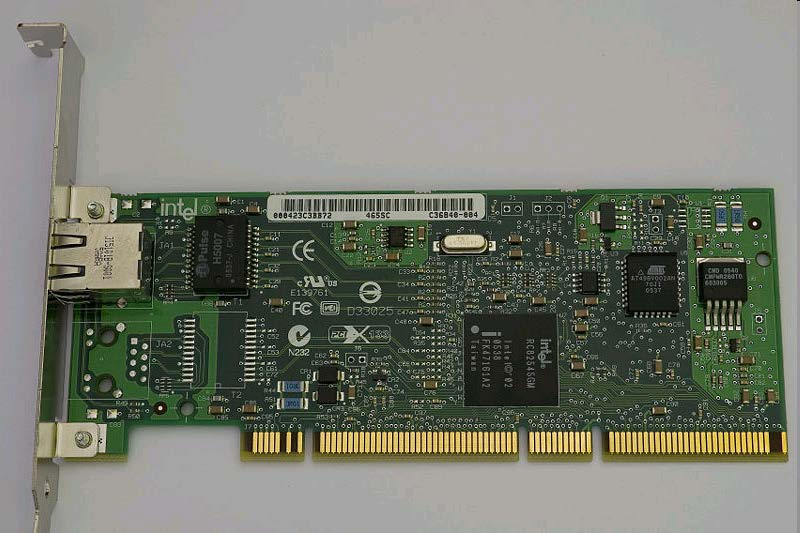
\includegraphics[width=0.5\linewidth]{extrahovane_obrazky/img_1_page16_3.jpeg}
	\end{center}
	
\end{frame}


\begin{frame}{Typy PCI a PCI - X}

    \begin{table}[]
        \begin{tabular}{|l|cc|cc|cc|}
        \hline
        Typ sběrnice        & \multicolumn{2}{c|}{PCI-33}    & \multicolumn{2}{c|}{PCI-66}    & \multicolumn{2}{c|}{PCI-X 66} \\ \hline
        Počet datových bitů & \multicolumn{1}{c|}{32}  & 64  & \multicolumn{1}{c|}{32}  & 64  & \multicolumn{1}{c|}{32}  & 64 \\ \hline
        Počet pinů          & \multicolumn{1}{c|}{49}  & 81  & \multicolumn{1}{c|}{49}  & 81  & \multicolumn{1}{c|}{50}  & 82 \\ \hline
        Přenosová rychlost MB/s & \multicolumn{1}{c|}{133} & 266 & \multicolumn{1}{c|}{266} & 533 & \multicolumn{1}{c|}{266} & 533 \\ \hline
        Napájecí napětí     & \multicolumn{2}{c|}{5V, 3,3 V} & \multicolumn{2}{c|}{5V, 3,3 V} & \multicolumn{2}{c|}{3,3 V}    \\ \hline
        \end{tabular}
    \end{table}

    \begin{table}[]
        \begin{tabular}{|cc|ccc|ccc|}
        \hline
        \multicolumn{2}{|c|}{PCI-X 133} & \multicolumn{3}{c|}{PCI-X 266}                         & \multicolumn{3}{c|}{PCI-X 533}                         \\ \hline
        \multicolumn{1}{|c|}{32}  & 64  & \multicolumn{1}{c|}{16} & \multicolumn{1}{c|}{32} & 64 & \multicolumn{1}{c|}{16} & \multicolumn{1}{c|}{32} & 64 \\ \hline
        \multicolumn{1}{|c|}{50}  & 82  & \multicolumn{1}{c|}{36} & \multicolumn{1}{c|}{50} & 82 & \multicolumn{1}{c|}{36} & \multicolumn{1}{c|}{50} & 82 \\ \hline
        \multicolumn{1}{|c|}{533} & 1066 & \multicolumn{1}{c|}{533} & \multicolumn{1}{c|}{1066} & 2133 & \multicolumn{1}{c|}{1066} & \multicolumn{1}{c|}{2133} & 4266 \\ \hline
        \multicolumn{2}{|c|}{3,3 V}     & \multicolumn{3}{c|}{1,5 V a 3,3 V}                     & \multicolumn{3}{c|}{1,5 V a 3,3 V}                     \\ \hline
        \end{tabular}
    \end{table}
\end{frame}

\section{AGP}
\begin{frame}{Interní port AGP}
	\begin{columns}
		\column{0.39\textwidth}
		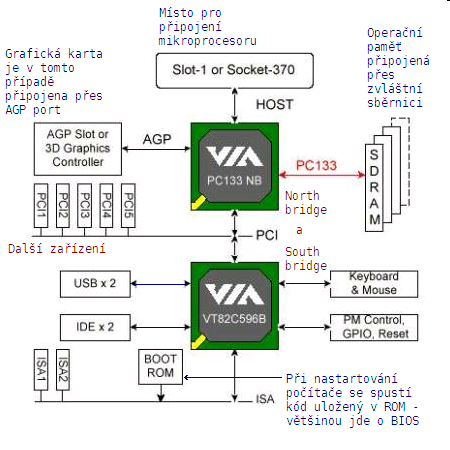
\includegraphics[width=1\linewidth]{extrahovane_obrazky/img_1_page18_0.png}
		\column{0.59\textwidth}
		\begin{itemize}
			\item AGP vzniklo zkrácením plného názvu Accelerated Graphics Port
			\item port určený prakticky výhradně k připojení grafických adaptérů
			\item technologie AGP vznikla úpravou sběrnice PCI
			\item frekvence hodinového signálu se zvýšila na 66 MHz
		\end{itemize}
        \begin{center}
            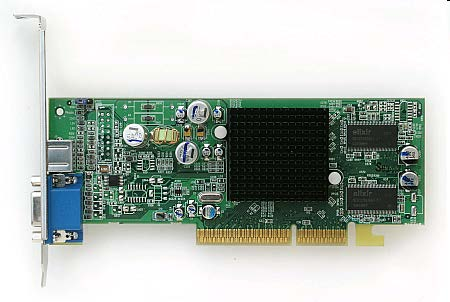
\includegraphics[width=0.8\linewidth]{extrahovane_obrazky/img_1_page18_15.jpeg}
        \end{center}
	\end{columns}
	
\end{frame}


\begin{frame}{}
	\begin{center}
		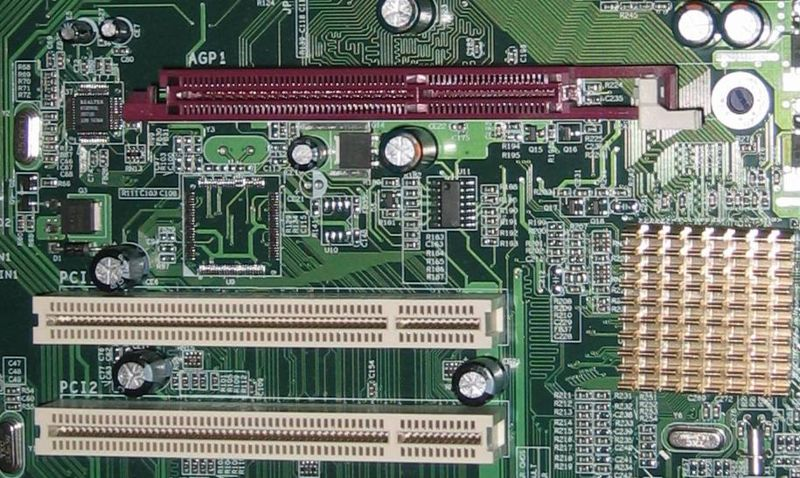
\includegraphics[width=0.8\linewidth]{extrahovane_obrazky/agp.jpeg}
	\end{center}
	
\end{frame}


\begin{frame}{Verze AGP}

    % První tabulka
    \begin{table}[]
        \begin{tabular}{|l|c|l|}
        \hline
        Verze   & Podporované rychlosti & Úroveň signálů   \\ \hline
        AGP 1.0 & 1× 2×                 & 3,3 V            \\ \hline
        AGP 2.0 & 1× 2× 4×              & 3,3 V nebo 1,5 V \\ \hline
        AGP Pro & 1× 2× 4×              & 3,3 V nebo 1,5 V \\ \hline
        AGP 3.0 & 1× 2× 4× 8× & \begin{tabular}[c]{@{}l@{}}1,5 V ovšem \\ pro rychlost 8× 0,8 V\end{tabular} \\ \hline
        \end{tabular}
    \end{table}
    
    \vspace{0.5cm}
    
    \begin{table}[]
        \begin{tabular}{|l|c|c|c|}
        \hline
        Označení & \begin{tabular}[c]{@{}c@{}}Hodinová \\ frekvence\end{tabular} & Režim přenosu & \begin{tabular}[c]{@{}c@{}}Výsledná \\ rychlost\end{tabular} \\ \hline
        AGP 1× & 66 MHz & 32 bitů za takt    & 266 MB/s  \\ \hline
        AGP 2× & 66 MHz & 2× 32 bitů za takt & 533 MB/s  \\ \hline
        AGP 4× & 66 MHz & 4× 32 bitů za takt & 1066 MB/s \\ \hline
        AGP 8× & 66 MHz & 8× 32 bitů za takt & 2133 MB/s \\ \hline
        \end{tabular}
    \end{table}
	
\end{frame}


\begin{frame}{}
	 
	\begin{center}
		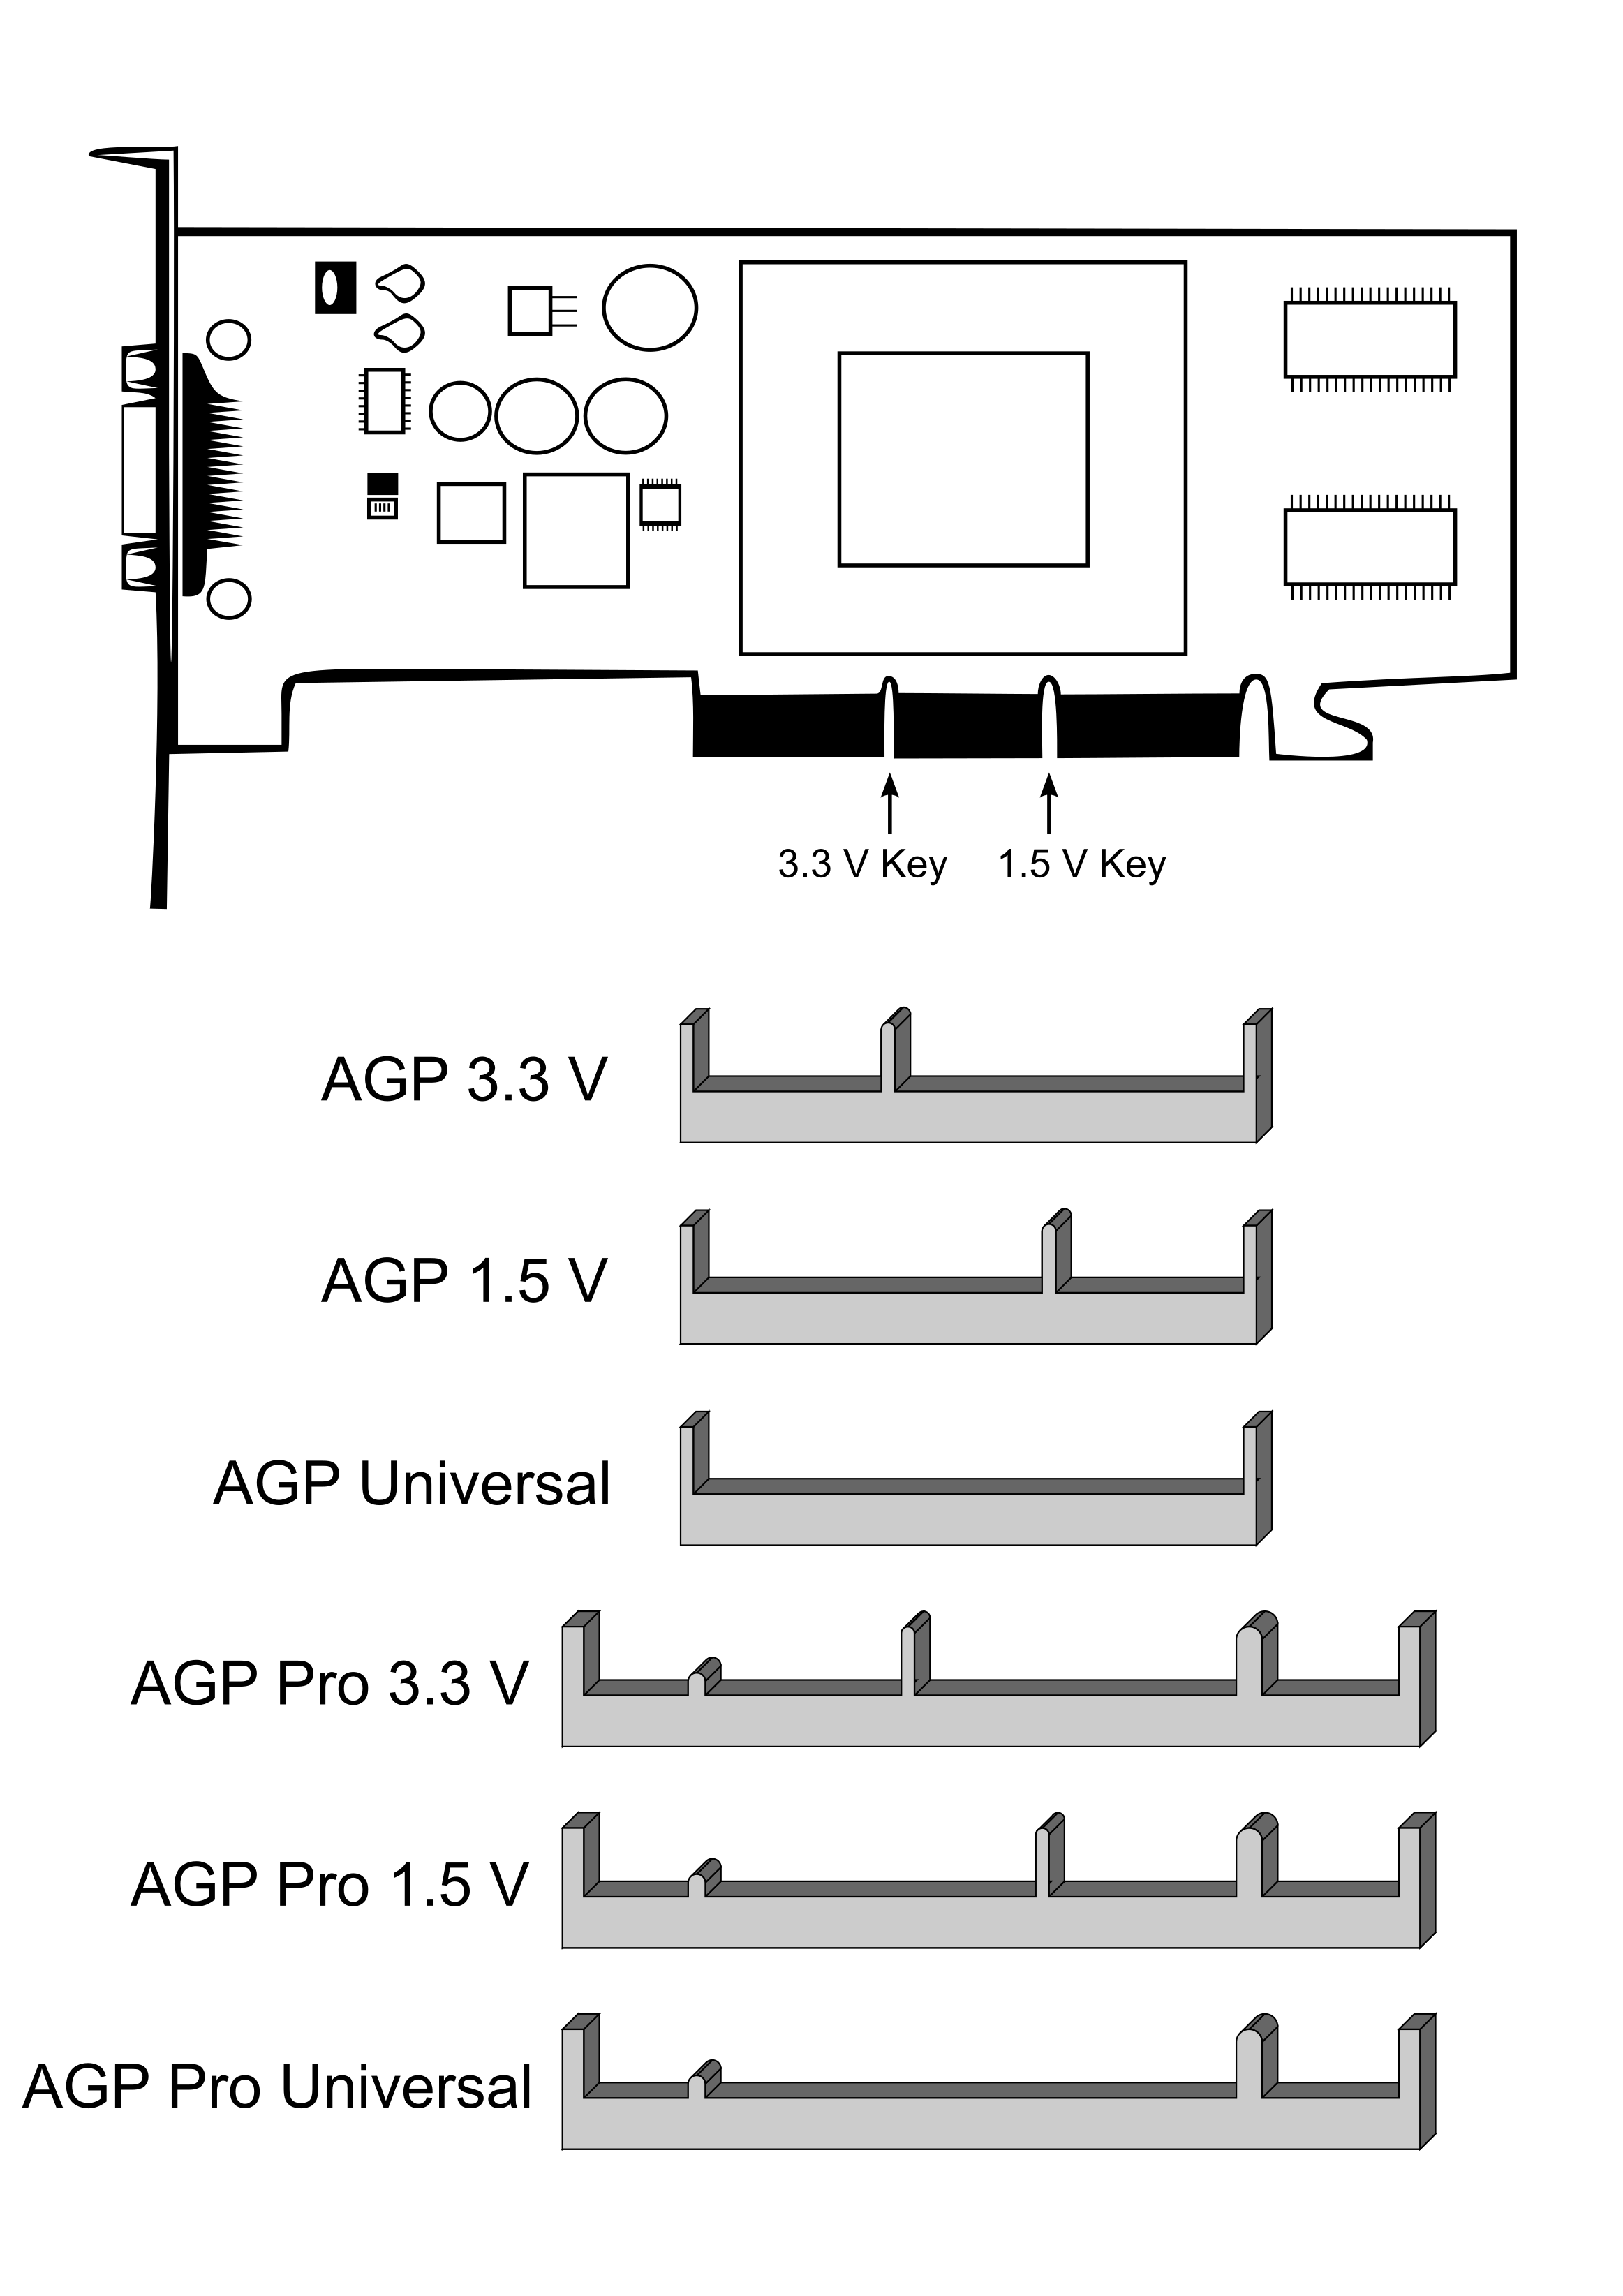
\includegraphics[width=0.55\linewidth]{extrahovane_obrazky/agp_k.png}
	\end{center}
	
\end{frame}

\section{AMR, CNR, ACR}
\begin{frame}{Další sběrnice - AMR, CNR, ACR}
	Karta PCI musí být plně osazena elektronickými obvody,což ji prodražuje. Levnější variatna:
	\begin{itemize}
		\item \textbf{AMR (Audio / Modem Riser)} je prvním standardem
		      tohoto typu, definovaným firmou Intel.
		      \begin{itemize}
		      	\item karty audio a faxmodemové.
		      	\item na základní desce jsou umístěny řídicí obvody, kdežto na samotné kartě AMR jsou jen přizpůsobovací obvody pro
		      	      konkrétní problematiku.
		      \end{itemize}
		\item \textbf{CNR (Communication and Networking Riser)}, firma Intel, řešení podporující navíc síťové karty. Bohužel toto řešení není zpětně kompatibilní s AMR.
		\item \textbf{ACR (Advanced Communications Riser)}, skupina výrobců (3Com, AMD, VIA a další) zavedla vlastní sběrnici, která vychází z AMR, a je s ní zpětně kompatibilní
	\end{itemize}
	
\end{frame}


\begin{frame}{Slot CNR}
	\begin{center}
		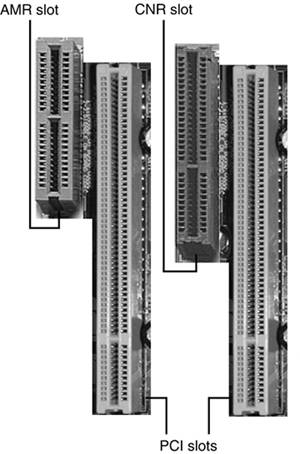
\includegraphics[width=0.45\linewidth]{extrahovane_obrazky/cnr.jpeg}
	\end{center}
	
\end{frame}


\begin{frame}{AMR}
	\begin{columns}
		\column{0.39\textwidth}
		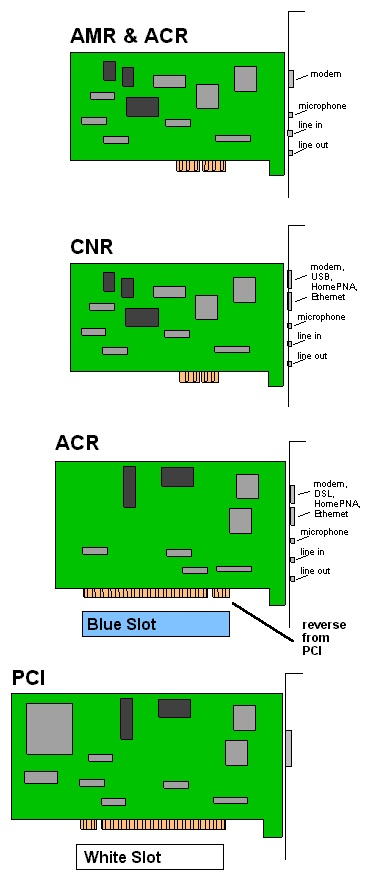
\includegraphics[width=0.65\linewidth]{extrahovane_obrazky/AMR_p.jpg}
		\column{0.59\textwidth}
		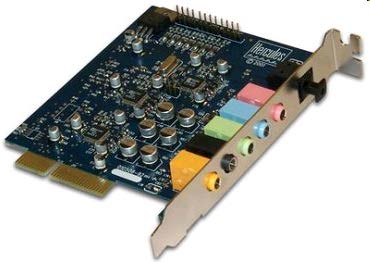
\includegraphics[width=1\linewidth]{extrahovane_obrazky/img_1_page25_1.jpeg}
	\end{columns}
\end{frame}

\section{PCI Ecpress}
\begin{frame}{Postupný vývoj sběrnic PCI, PCI-X a PCI Express}
	
	\begin{center}
		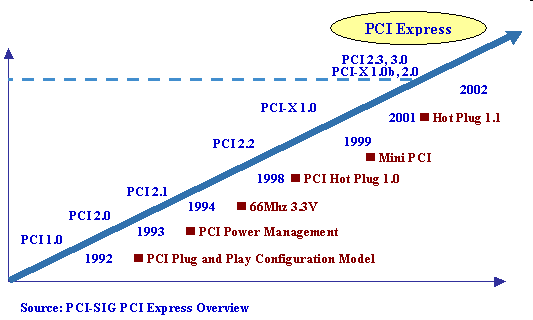
\includegraphics[width=1\linewidth]{extrahovane_obrazky/img_2_page1_0.png}
	\end{center}
\end{frame}


\begin{frame}{PCI Express}
	\begin{itemize}
		\item sériová, resp. sério-paralelní, plně duplexní
		\item PCI Express vychází spíše ze sítí typu peer-to-peer než z architektury PCI nebo PCI-X (podobnost s ISO-OSI).
		\item Architektura typu peer-to-peer umožňuje nezávislou komunikaci mezi jednotlivými zařízeními, kdy jedno zařízení nemusí čekat na uvolnění sběrnice při vzniku požadavku na komunikaci s jiným zařízením, jak tomu bylo u architektury PCI.
	\end{itemize}
	
\end{frame}


\begin{frame}{Vrstvy sběrnice PCI Express}
	 
	\begin{center}
		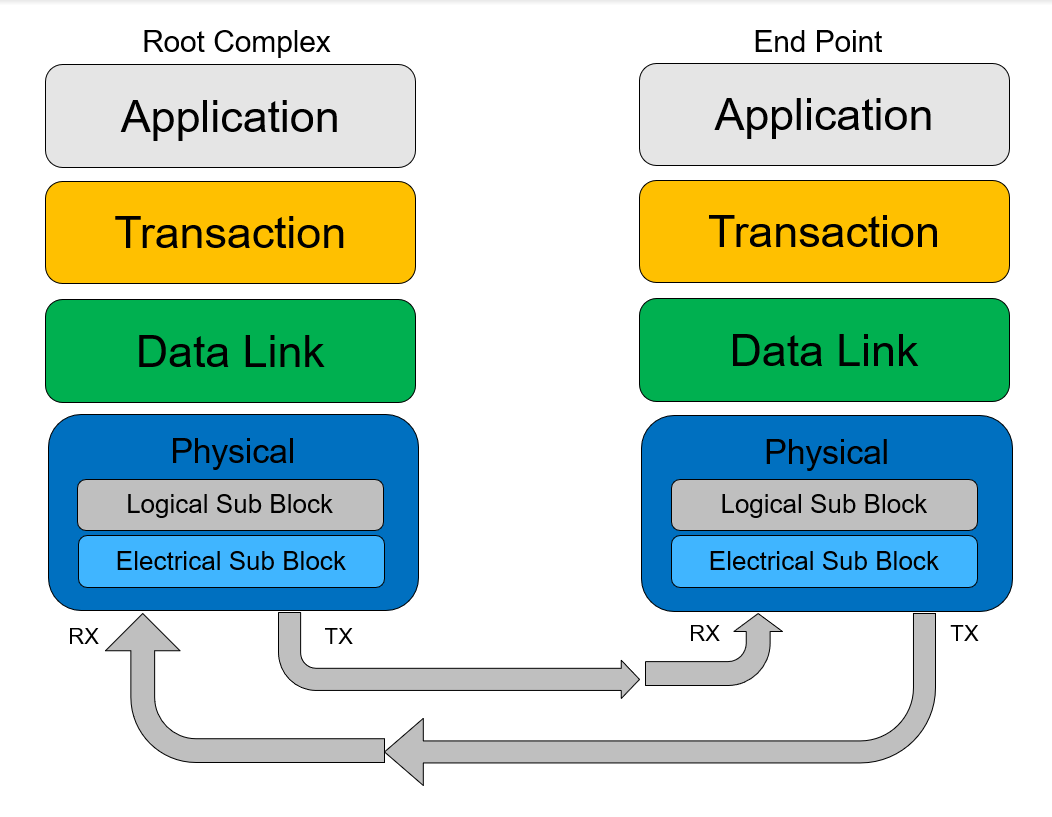
\includegraphics[width=0.85\linewidth]{extrahovane_obrazky/pcie_l.png}
	\end{center}
\end{frame}

\begin{frame}{Vrstvy sběrnice PCI Express}
	 
	\begin{itemize}
		\item Fyzická vrstva (Physical Layer)
		      \begin{itemize}
		      	\item konektory, signálové cesty
		      	\item linky (lanes) - 2 diff. páry
		      \end{itemize}
		\item Linková vrstva (Data Link Layer)
		      \begin{itemize}
		      	\item bezchybný přenos - CRC a opakování přenosu
		      	\item data ve frame-ech
		      \end{itemize}
		\item Transakční vrstva (Transaction Layer)
		      \begin{itemize}
		      	\item komunikace zařízení - procesor
		      	\item řízení přístupu k pamětí (DMA)
		      \end{itemize}
		\item Protokolová vrstva (Software Layer)
		      \begin{itemize}
		      	\item HW a OS
		      \end{itemize}
	\end{itemize}
\end{frame}

\begin{frame}{Základy technologie PCI Express}
	\begin{itemize}
		\item dva páry vodičů
		\item každý pár vodičů přitom provádí přenos v jednom směru s rychlostí 2,525 Gb/s (u verze 2 je to dvojnásobek).
	\end{itemize}
	
	\begin{center}
		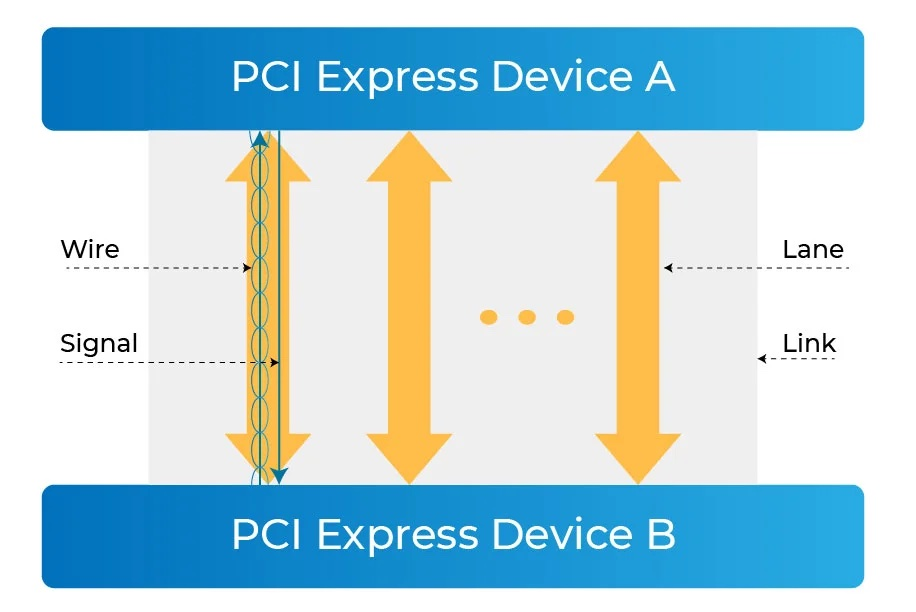
\includegraphics[width=0.8\linewidth]{extrahovane_obrazky/pci_laL.jpg}
	\end{center}
	
\end{frame}


\begin{frame}{Základy technologie PCI Express}
	\begin{itemize}
		\item 2x lane = LINK (obousměrně)
		\item proudová smyčka - rychlosti a rušení
	\end{itemize}
	
	\begin{columns}
		\column{0.49\textwidth}
		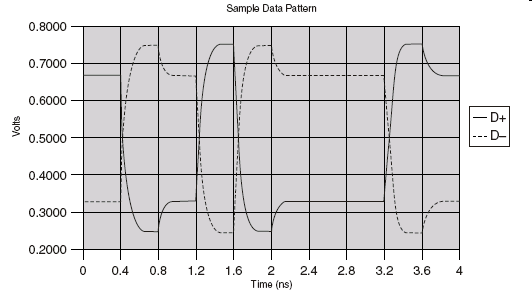
\includegraphics[width=1\linewidth]{extrahovane_obrazky/img_2_page5_14.png}
		\column{0.49\textwidth}
		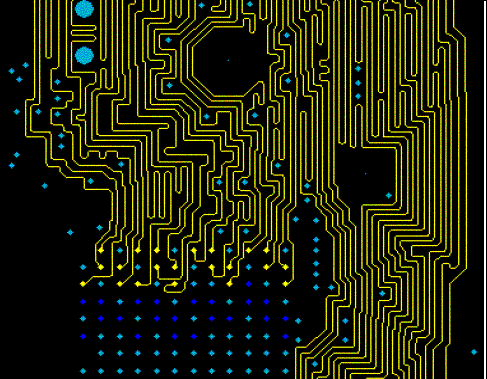
\includegraphics[width=1\linewidth]{extrahovane_obrazky/img_2_page5_15.png}
	\end{columns}
	
\end{frame}


\begin{frame}{Diferenciální datový pár}
	 
	\begin{center}
		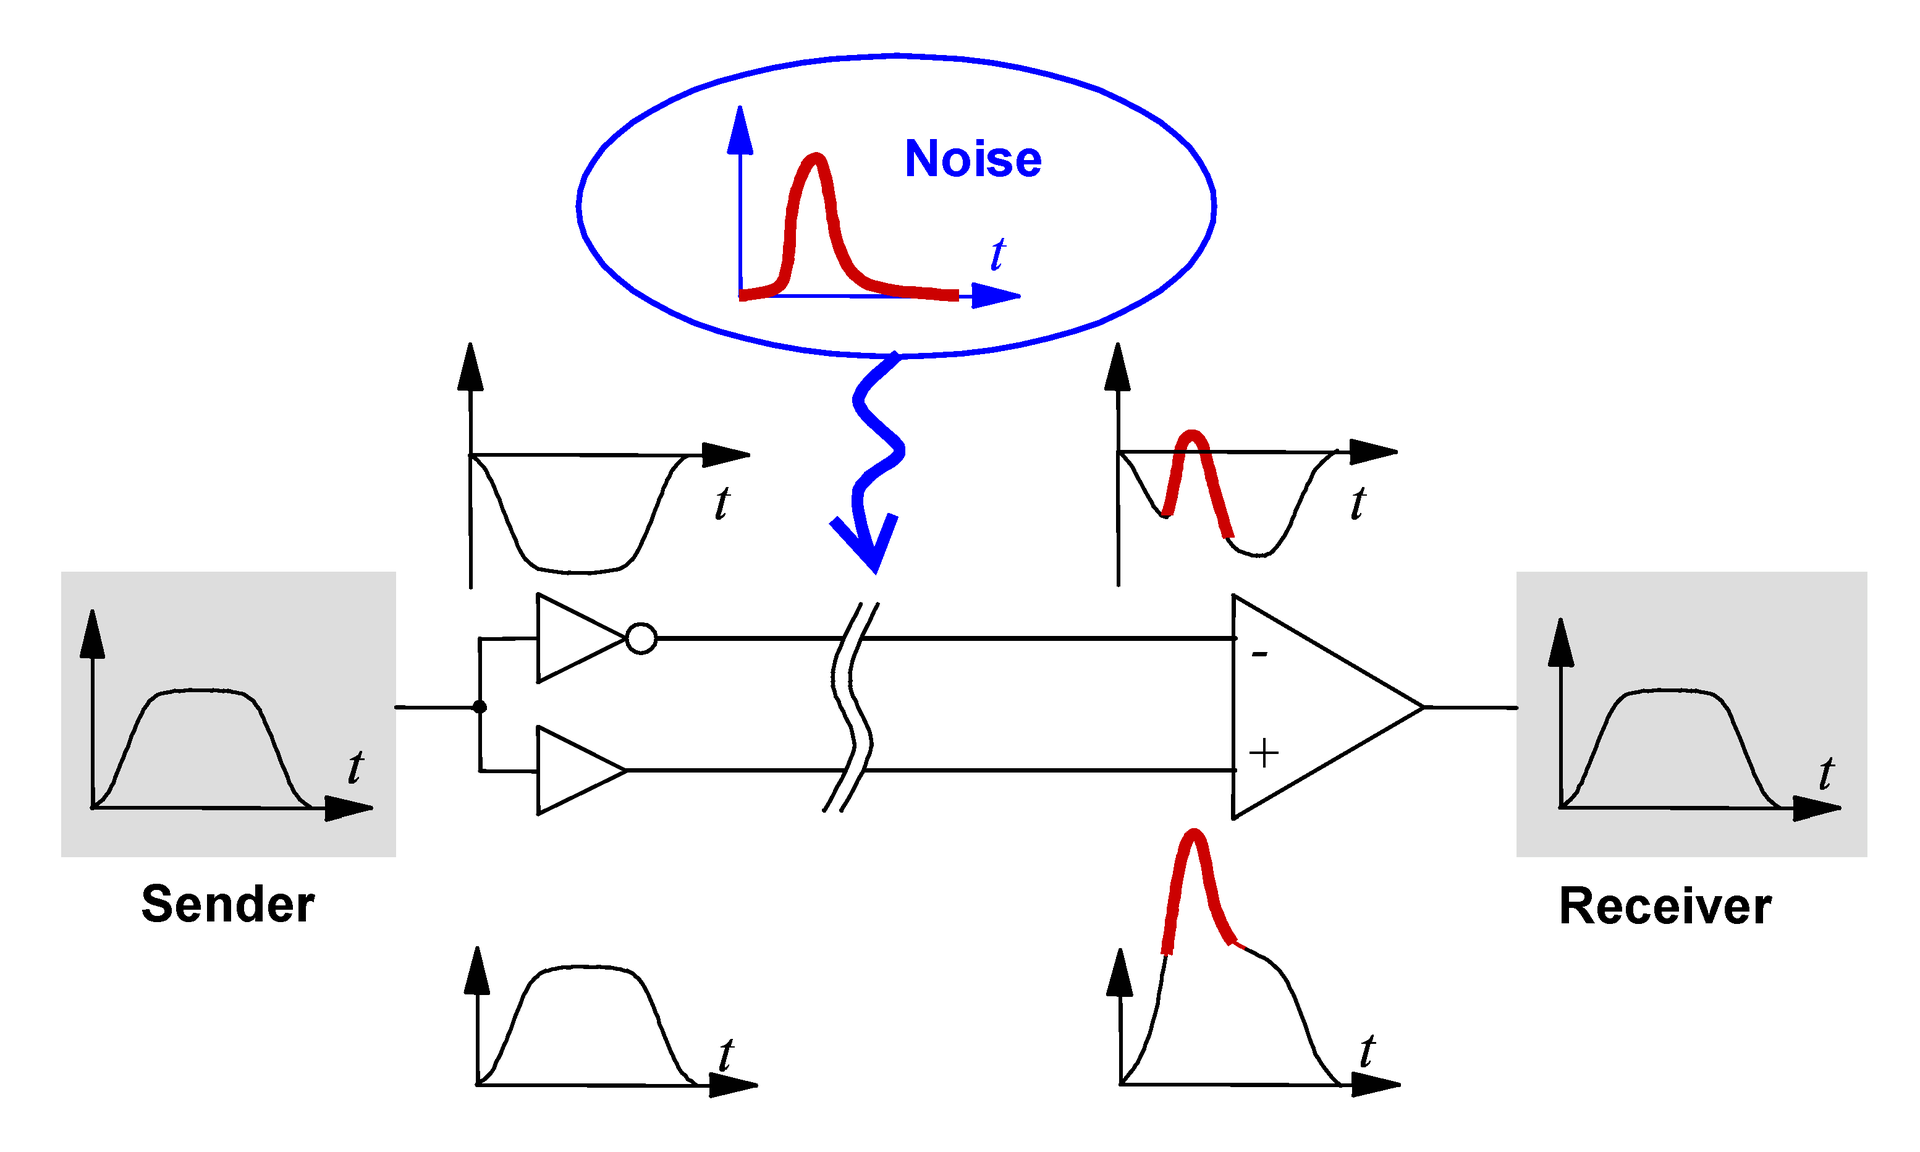
\includegraphics[width=1\linewidth]{extrahovane_obrazky/diff.png}
	\end{center}
	
\end{frame}


\begin{frame}{PCI Express Link}
	
	\begin{columns}
		\column{0.39\textwidth}
		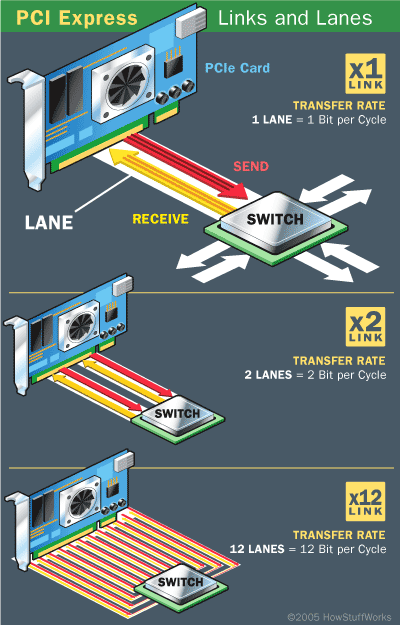
\includegraphics[width=1\linewidth]{extrahovane_obrazky/img_2_page7_0.png}
		\column{0.59\textwidth}
		\begin{itemize}
			\item PCI Express Link reprezentuje komunikační kanál mezi dvěma zařízeními sběrnice PCI Express
			\item Základní PCI Express Link je sestaven ze dvou nízkonapěťových diferenciálních párů a to přijímacího a vysílacího datového páru označovaného jako Lane.
			\item Činnost vysílače i přijímače je na sobě nezávislá a Link tvoří plně duplexní komunikační kanál.
			\item Lane tedy označuje 2 datové páry, každý v opačném směru.
		\end{itemize}
	\end{columns}
	
\end{frame}


\begin{frame}{Základní vlastnosti komunikačního kanálu}
	\begin{itemize}
		\item Základní link se skládá ze dvou jednosměrných diferenciálních párů, každý v jednom směru, reprezentující přijímací a vysílací pár = 1 Lane.
		\item Hodinový signál je kódovaný do datového toku, aby mohlo být dosaženo maximální přenosové rychlosti.
		\item Každý link může pracovat s příslušnými signálovými úrovněmi pro které byl navržen.
		\item Přenosová rychlost je závislá na verzích specifikace.
	\end{itemize}
	
\end{frame}


\begin{frame}{Varianty PCI Express}
	\begin{itemize}
		\item Každý Link musí podporovat alespoň jeden Lane
		\item Pro zvýšení přenosové rychlosti je možné využít sdružování Lanes do Linků v povolené šířce.
		\item Obvykle se jedná o hodnoty x1, x2, x4, x8, x12, x16 a x32.
		\item Stejná šířka musí byt dodržena jak pro přijímací, tak vysílací část.
		\item Během hardwarové inicializace Linku se vyjedná pracovní frekvence a počet Lanes sestavujících Link. (Obdoba vyjednávání pracovní frekvence sítí typu Ethernet.)
	\end{itemize}
	
\end{frame}


\begin{frame}{PCI Express}
	\begin{columns}
		\column{0.39\textwidth}
		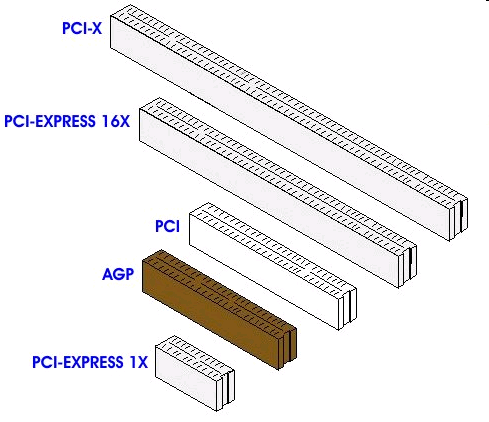
\includegraphics[width=1\linewidth]{extrahovane_obrazky/img_2_page11_43.png}
		\column{0.59\textwidth}
		\begin{itemize}
			\item Karta určená do sběrnice PCI Express ×1, kterou je však možné zapojit i do všech širších konektorů PCI Express – ×2, ×4, ×8 i ×16
			      \itemU karet, které vyžadují větší datové toky (například se jedná o grafické akcelerátory), je možné použít několika linků současně zavedených do jednoho konektoru.
			\item Podle počtu linků se takové konektory a karty označují: PCI e  ×1, x2,×4, ×8, ×12, ×16, ×32.
		\end{itemize}
	\end{columns}
	
\end{frame}


\begin{frame}{}
	 
	\begin{center}
		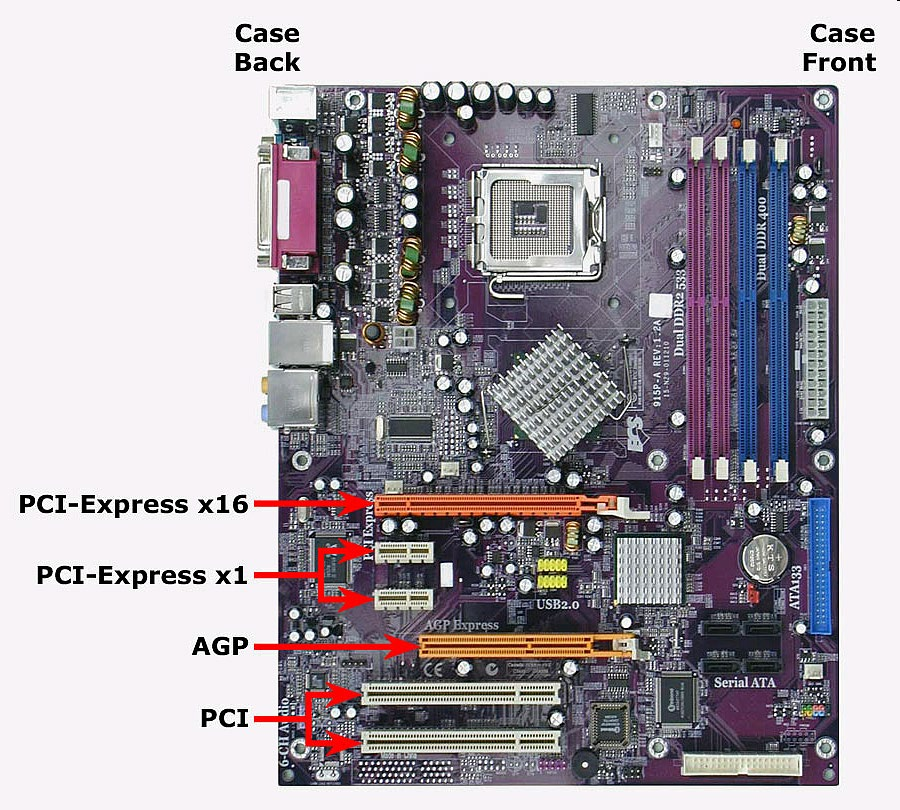
\includegraphics[width=0.8\linewidth]{extrahovane_obrazky/img_2_page12_0.jpeg}
	\end{center}
	
\end{frame}

\begin{frame}{}
	 
	\begin{center}
		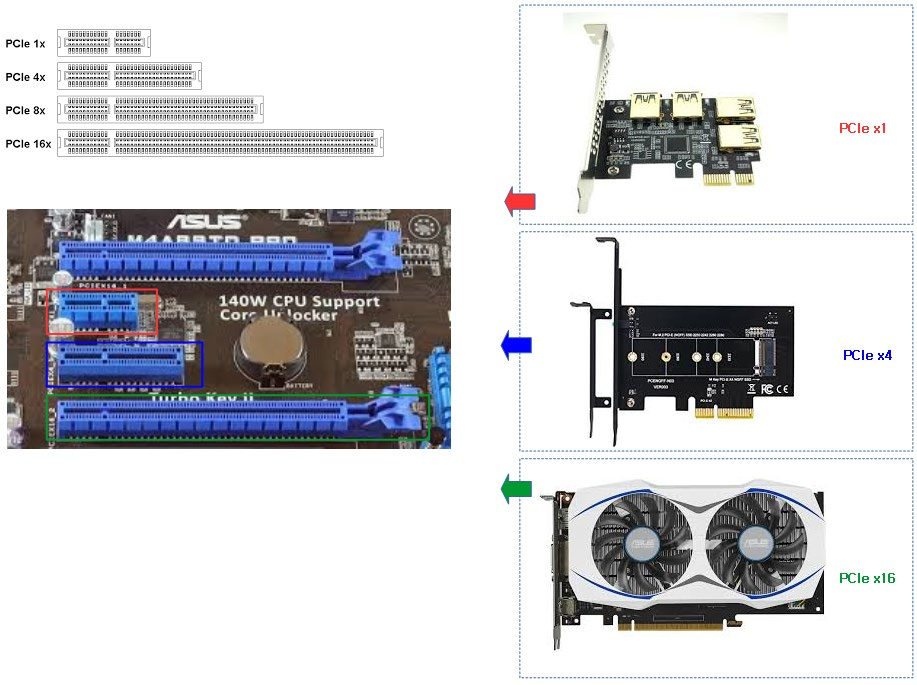
\includegraphics[width=1\linewidth]{extrahovane_obrazky/img_2_page14_0.jpeg}
	\end{center}
	
\end{frame}


\begin{frame}{Přenosová rychlost PCIe}
	\begin{itemize}
		\item jeden Link - dosaženo přenosové rychlosti cca 250 MB.s-1 v každém směru (ve verzi 1 - reálná přenosová rychlost bude o cca 5 procent nižší, protože je nutné přenášet i řídicí sekvence, opravné kódy atd.)
		\item 2,525 Gb/s $\neq$ 250 MB/s - správná jednotka je totiž GT/s  (tedy 2,5 GT/s) – protože toto číslo zahrnuje i servisní bity
		\item kódování 8/10 tj. každých osm bitů surových dat je převedeno na deset bitů, přičemž je zajištěna maximální délka sekvence nul a jedniček – to je nutné pro synchronizaci přenosu na tak vysokých rychlostech, i když se tím přenosové pásmo sníží o 25\%.
	\end{itemize}
	
\end{frame}


\begin{frame}{Verze PCI Express}
	\begin{itemize}
		\item Verze 1.Oa - rok 2003 a Verze 1.1 rok 2005
		      \begin{itemize}
		      	\item rychlost 250 MB/s v jednom směru (500 MB/s obousměrně), jsou vzájemně kompatibilní
		      \end{itemize}
		\item Verze 2.O
		      \begin{itemize}
		      	\item rychlost 500 MB/s v jednom směru (1 GB/s obousměrně)
		      	\item tato verze je zpětně i dopředně kompatibilní, lze tedy karty s podporou PCI- Express 2.0 zapojit do základní desky, která obsahuje pouze podporu verze 1.1 a naopak
		      \end{itemize}
		\item Verze 2.1
		      \begin{itemize}
		      	\item rychlost 500 MB/s v jednom směru (1 GB/s obousměrně)
		      	\item navýšení napájení slotu - přerušení zpětné kompatibility mezi verzemi 2.1 a 1.0a
		      	\item  pro většinu základních desek s PCIe 1.1 existují aktualizace systémů BIOS od jejich výrobců, díky kterým je zpětná kompatibilita zajištěna
		      \end{itemize}
	\end{itemize}
	
\end{frame}
\begin{frame}{Verze PCI Express}
	\begin{itemize}
		\item Verze 3.0
		      \begin{itemize}
		      	\item rychlost 1 GB/s v jednom směru (2 GB/s obousměrně)
		      	\item Namísto odstraněného 8b/10b je zde použito 128b/130b kódovací schéma - režie při přenosu dat klesla z původních 20\% u PCIe 2.0 přibližně na 1,5\%
		      	\item 8 GT/s
		      \end{itemize}
		\item Verze 4.0
		      \begin{itemize}
		      	\item rychlost 2 GB/s v jednom směru (4 GB/s obousměrně)
		      	\item 16 GT/s
		      \end{itemize}
		\item Verze 5.0 (2019)
		      \begin{itemize}
		      	\item rychlost 4 GB/s v jednom směru (8 GB/s obousměrně)
		      	\item 32 GT/s
		      \end{itemize}
	\end{itemize}
	
\end{frame}

\begin{frame}{PCIe ver.1 a ver. 2}
	 
	\begin{center}
		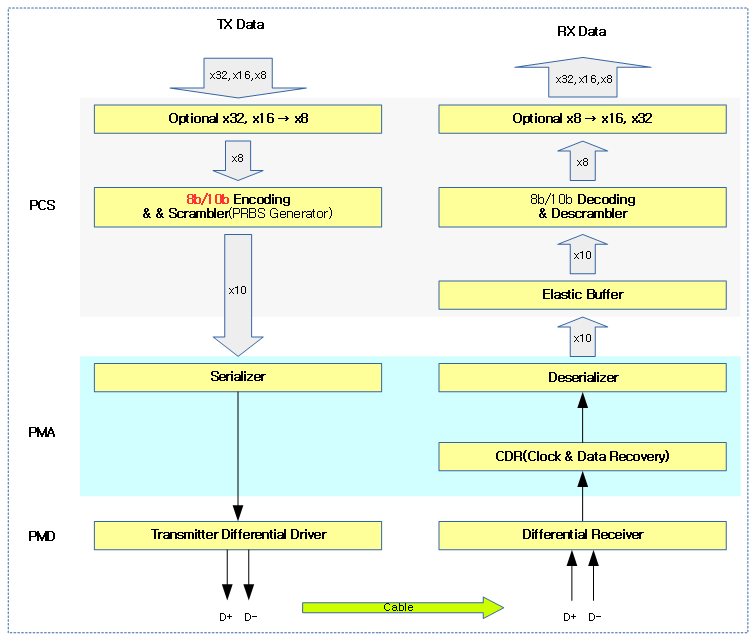
\includegraphics[width=0.8\linewidth]{extrahovane_obrazky/img_2_page17_2.png}
	\end{center}
	
\end{frame}

\begin{frame}{PCIe ver.3, ver. 4 a ver. 5}
	 
	\begin{center}
		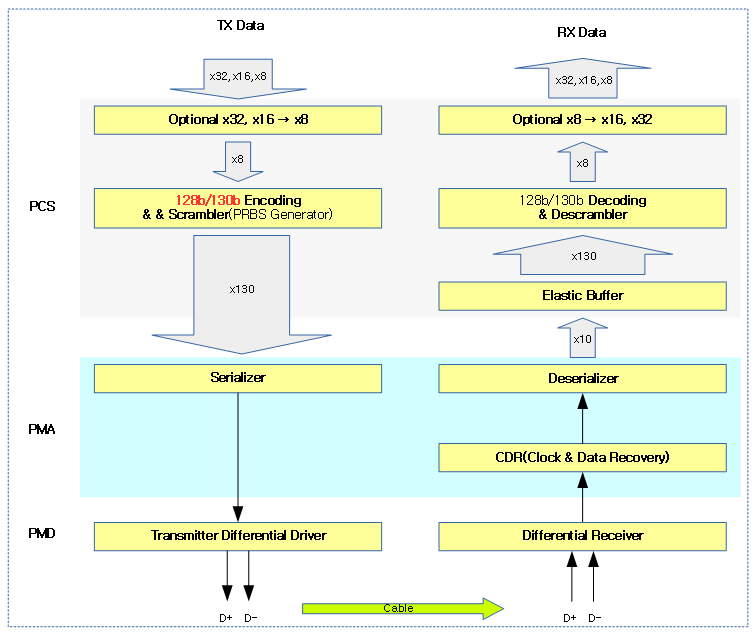
\includegraphics[width=0.8\linewidth]{extrahovane_obrazky/img_2_page20_0.png}
	\end{center}
	
\end{frame}



\begin{frame}{PCI Express 6.0 (2022)}
	\begin{itemize}
		\item rychlost 7,9 GB/s v jednom směru
		\item 64 GT/s
		\item PCIe 6.0 pracuje stejně jako PCIe 5.0 na frekvenci 32 GHz, liší se však modulací signálu. Opouští původní NRZ (Non Return to Zero) na PAM4 (Pulse-Amplitude Modulation 4).
		\item Vylepšená oprava chyb (FEC)s nízkou latencí.
		\item PCIe zůstává zpětně kompatibilní s předchozími verzemi rozhraní
	\end{itemize}
	\begin{center}
		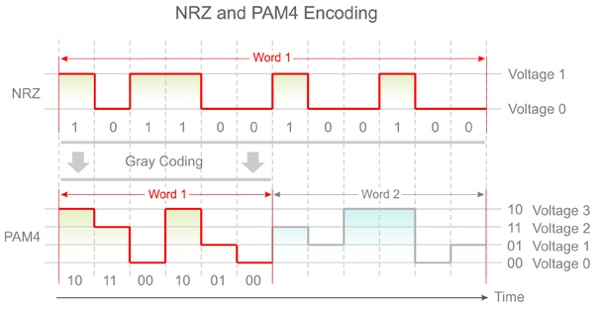
\includegraphics[width=0.7\linewidth]{extrahovane_obrazky/pam4.jpg}
	\end{center}
	
\end{frame}

\begin{frame}{PCI Express 7.0 (2023)}
\begin{itemize}
    \item rychlost 15,8 GB/s v jednom směru
    \item 128 GT/s
    \item Používá stejnou PAM4 modulaci jako PCIe 6.0
    \item Další vylepšení v oblasti spolehlivosti a latence
    \item Zachovává zpětnou kompatibilitu
    \item Očekávaná dostupnost v produktech: 2025
\end{itemize}
\end{frame}

\begin{frame}{Srovnání PCE Express}
	\begin{table}[]
        \begin{tabular}{|l|c|c|c|c|}
        \hline
        \textbf{Rozhraní} & \textbf{Propustnost} & \textbf{Kódování} & \textbf{Rychlost ×1} & \textbf{Uvedení} \\ \hline
        PCIe 1.0 & 2,5 GT/s & 8b/10b    & 250 MB/s  & 2003 \\ \hline
        PCIe 2.0 & 5 GT/s   & 8b/10b    & 500 MB/s  & 2007 \\ \hline
        PCIe 3.0 & 8 GT/s   & 128b/130b & 985 MB/s  & 2010 \\ \hline
        PCIe 4.0 & 16 GT/s  & 128b/130b & 1,97 GB/s & 2017 \\ \hline
        PCIe 5.0 & 32 GT/s  & 128b/130b & 3,94 GB/s & 2019 \\ \hline
        PCIe 6.0 & 64 GT/s  & PAM4      & 7,88 GB/s & 2022 \\ \hline
        PCIe 7.0 & 128 GT/s & PAM4 & 15,76 GB/s & 2023 \\ \hline
        \end{tabular}
    \end{table}
	
\end{frame}


\begin{frame}{Základní deska}
	\begin{columns}
		\column{0.59\textwidth}
		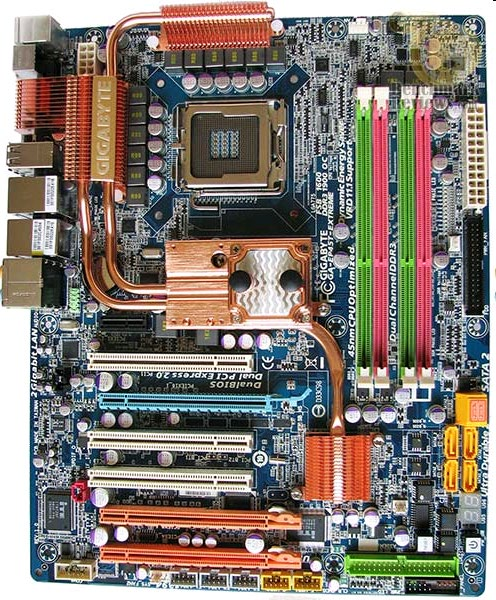
\includegraphics[width=0.8\linewidth]{extrahovane_obrazky/img_2_page24_0.jpeg}
		\column{0.39\textwidth}
		\begin{itemize}
			\item jeden konektor PCI Express ×16 (modrý)
			\item dva konektory ×8 (oranžové)
			\item jeden konektor ×1 (černý)
			\item tři klasické konektory PCI sběrnice (bílé).
		\end{itemize}
	\end{columns}
	
\end{frame}


\begin{frame}{Konektor není specifikace}
	Někdy  konektory ×16 ve skutečnosti pracují v režimu ×8, což je případ některých základních desek, které obsahují dva „×16“ konektory určené
	pro grafické karty. Toto je omezení hardwarové přenosové šířky sběrnice.
	\begin{center}
		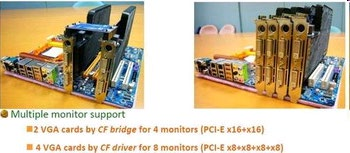
\includegraphics[width=0.8\linewidth]{extrahovane_obrazky/img_2_page25_0.jpeg}
	\end{center}
	
\end{frame}


\begin{frame}{Konektor není specifikace}
	Z87 z platformy LGA1150. U ní má procesor k dispozici pouze 16 linek PCI-E standardu 3.0. Konfigurace PCI-E linek může být buď 1× 16, 2× 8 nebo 8+4+4 (teoreticky).\\
	Základ je tedy pouze 1× 16 a 2× 8 linek. Pokud osadíte do prvního
	slotu grafiku a do druhého PCI-E disk, pojede obojí pouze na 8 PCI-E linek. Nutné podotknout že pojedeme podle nejnižší verze (2.0 + 3.0 = 2.0).
	
	\begin{center}
		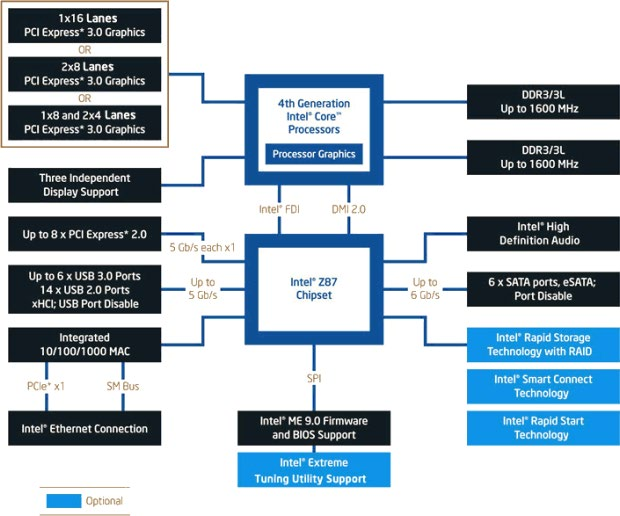
\includegraphics[width=0.5\linewidth]{extrahovane_obrazky/img_2_page26_0.jpeg}
	\end{center}
	
\end{frame}



\begin{frame}{Komunikace po PCI Express}
	\begin{itemize}
		\item U PCI Express není použita klasická sběrnicová topologie, u které jednotlivé karty musí žádat o přístup na sběrnici a sdílet přenosové pásmo s ostatními zařízeními.
		\item Místo toho vedou od všech konektorů jednotlivé dráhy do přepínače (switch), který (teoreticky) dokáže libovolné dvě dráhy propojit a vytvořit tak strukturu typu point-to-point.
	\end{itemize}
	
\end{frame}


\begin{frame}{Zařízení sběrnice PCI Express}
	PCI Express je sestavena ze zařízení, která jsou vzájemně propojena a zajišťují nezbytné funkce sběrnice :
	\begin{itemize}
		\item \textbf{root complex} - je začátkem sběrnice, propojujícím sběrnice s mikroprocesorem a řadičem operační paměti. Dále zajišťuje konfiguraci celé sběrnice .
		\item \textbf{Switches} - zajišťuje větvení a rozšiřování sběrnice PCI Express od Root Complexu nebo switche k dalším zařízením PCI Express (End Pointy, Switche a Bridge).
		\item \textbf{Bridges} - obstarává převod mezi PCI Express a jiným typem sběrnice (PCI, PCI-X nebo jiným)
		\item \textbf{Endpoints} - koncová zařízení, k nimž (z nichž) proudí data
	\end{itemize}
	
\end{frame}


\begin{frame}{}
	 
	\begin{center}
		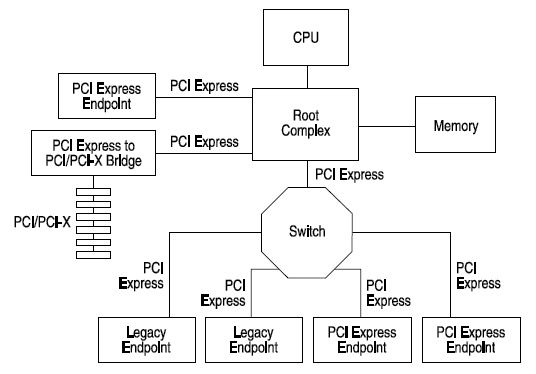
\includegraphics[width=1\linewidth]{extrahovane_obrazky/img_2_page30_0.png}
	\end{center}
	
\end{frame}


\begin{frame}{}
	 
	\begin{center}
		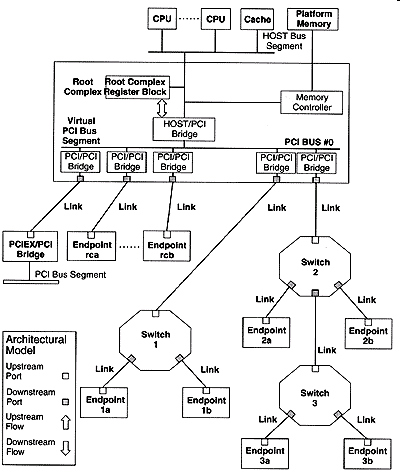
\includegraphics[width=0.6\linewidth]{extrahovane_obrazky/img_2_page31_0.png}
	\end{center}
	
\end{frame}


\begin{frame}{Komunikace po PCI Express}
	\begin{itemize}
		\item na základní desce musí být poměrně složitý přepínač, na stranu druhou však odpadá arbitrážní obvod (přiděluje přístup)
		\item každý link může přenášet data maximální rychlostí a zařízení se tak nemusí dělit o jedno přenosové pásmo (např. PCI)
		\item Proč se však stále mluví o „sběrnici“, když je použita jiná topologie? Na úrovni řízení se totiž ovládacím programům zařízení skutečně jeví tak, jako by byla připojena na sběrnici, i když se na úrovni vlastních vodičů o sběrnici nejedná. (podobně USB)
		      
	\end{itemize}
	
\end{frame}

\section{PCI Express dnes}
\begin{frame}{Moderní využití PCIe}
    \begin{columns}
        \column{0.6\textwidth}
        \begin{itemize}
            \item \textbf{NVMe SSD}
                \begin{itemize}
                    \item Využívají PCIe pro přímé připojení k CPU
                    \item PCIe 4.0 x4: až 7.88 GB/s
                    \item PCIe 5.0 x4: až 15.76 GB/s
                \end{itemize}
            \item \textbf{Grafické karty}
                \begin{itemize}
                    \item PCIe 4.0 x16: až 31.5 GB/s
                    \item PCIe 5.0 x16: až 63 GB/s
                    \item Podpora resizable BAR pro lepší využití paměti
                    \begin{itemize}
                        \item Bez reBAR: Když hra potřebuje načíst 8GB texturu, musí ji posílat po 256MB kusech
                        \item S reBAR: Celá 8GB textura může být přenesena v jedné operaci
                    \end{itemize}
                \end{itemize}
        \end{itemize}
        \column{0.4\textwidth}
        \begin{center}
            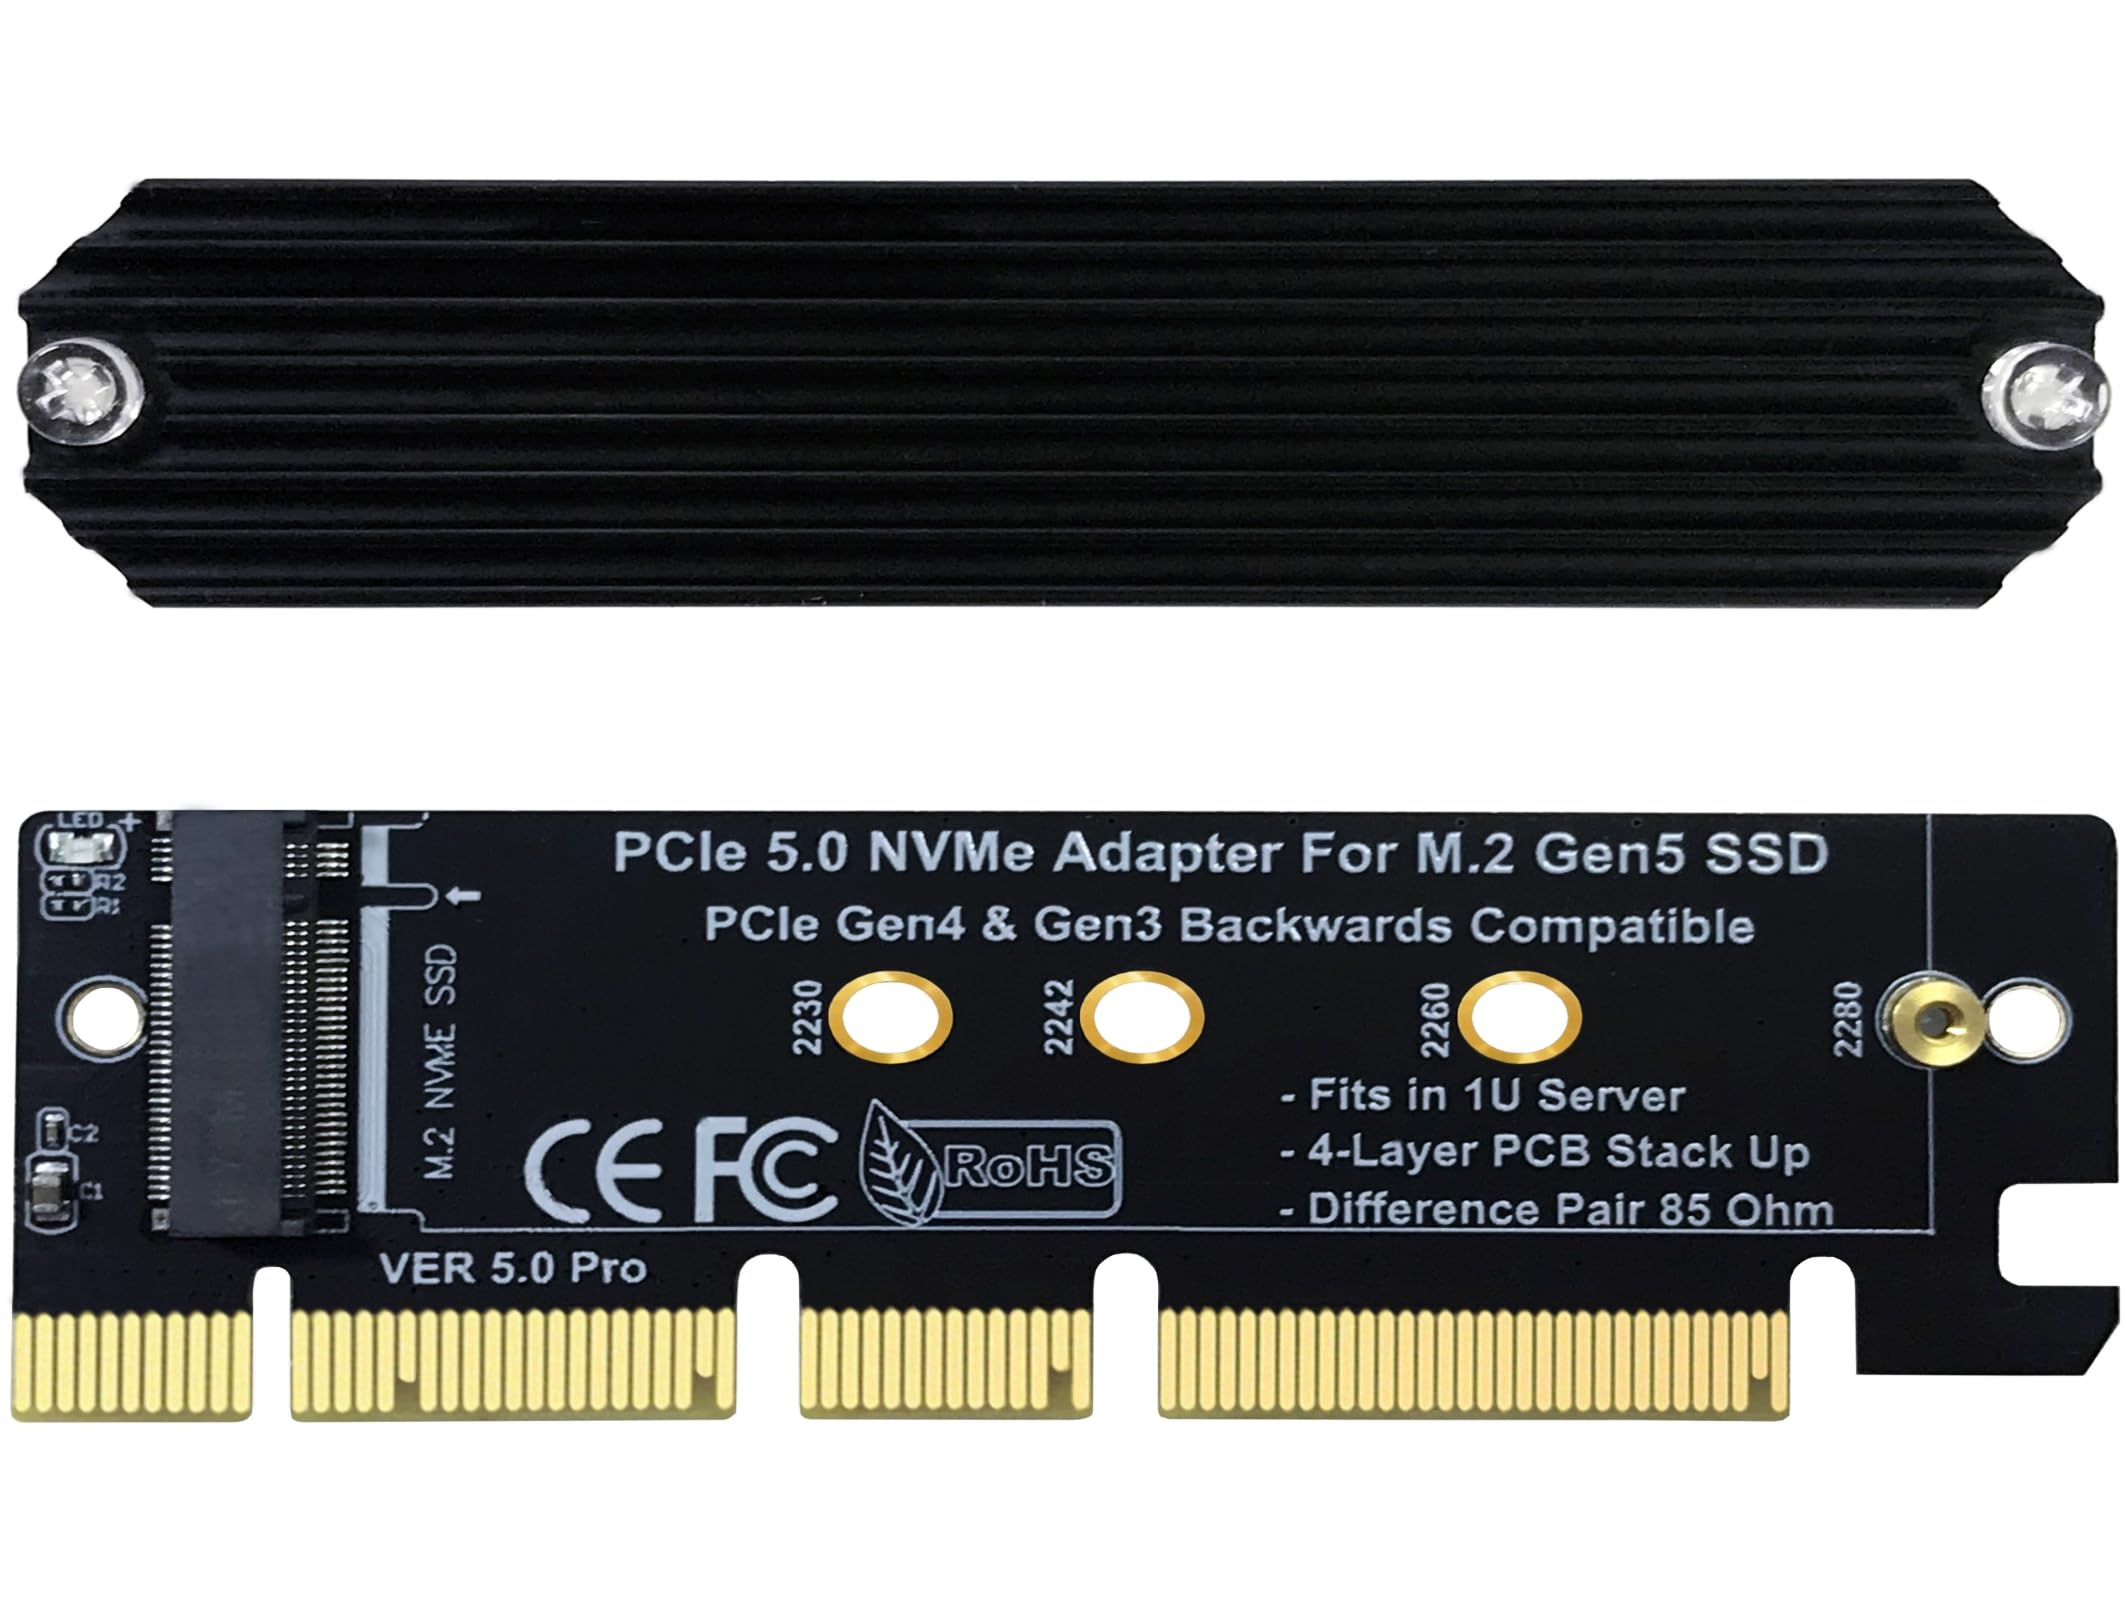
\includegraphics[width=1\linewidth]{extrahovane_obrazky/nvme.jpeg}
        \end{center}
    \end{columns}
\end{frame}

\begin{frame}{Nové technologie postavené na PCIe}
    \begin{itemize}
        \item \textbf{CXL (Compute Express Link)}
            \begin{itemize}
                \item Postaveno na fyzické vrstvě PCIe
                \item Umožňuje koherentní přístup k paměti mezi CPU a akcelerátory (bez RAM)
                \item Využití v AI/ML akcelerátorech a vysokovýkonných SSD
                \item CXL 3.0 podporuje sdílenou paměť až 2PB
            \end{itemize}
        \item \textbf{DirectStorage}
            \begin{itemize}
                \item Technologie pro rychlejší načítání her
                \item Přímý přenos dat z NVMe SSD do GPU paměti
                \item Snížení latence a zatížení CPU
                \item Vyžaduje PCIe 4.0 nebo novější
            \end{itemize}
        \item \textbf{PCIe jako univerzální rozhraní}
            \begin{itemize}
                \item Síťové karty 100/200/400 Gb/s
                \item AI akcelerátory
                \item Specializované výpočetní karty
            \end{itemize}
    \end{itemize}
\end{frame}

\section{Zdroje}
\begin{frame}{Použité zdroje}
    Prezentace vychází z prezentací Ing. Ralbovského a jedná se o jejich spojení, úpravu a případné aktualizace dat.
    \scriptsize
    \begin{itemize}
        \item HORÁK, Jaroslav. Hardware učebnice pro pokročilé. Brno: CPRESS, 2007, ISBN 978-80-251-1741-5.
        \item DEMBOWSKI, Klaus. Mistrovství v HARDWARU. Brno: CPRESS, 2009, ISBN 978-80-251-2310-2.
        \item TIŠŇOVSKÝ, Pavel. Interní sběrnice PCI Express [online]. [cit. 19.8.2013].
        \item AUTOR NEUVEDEN. PCI Express - mýty a fakta [online]. [cit. 20.8.2013].
        \item AUTOR NEUVEDEN. PCI Express [online]. [cit. 20.8.2013].
        \item PŮHONÝ, Jan. PCI-Express – obecný popis [online]. [cit. 20.8.2013].
        \item AUTOR NEUVEDEN. Rozhraní PCI Express 5.0 hotové, dvakrát rychlejší uvedení [online].
        \item AUTOR NEUVEDEN. PCI-SIG zveřejnil finální specifikace PCI Express 5.0 [online].
        \item AUTOR NEUVEDEN. PCI Express 6.0 opět zdvojnásobí rychlost [online].
        \item PCI-SIG. PCI Express 7.0 Specification to Deliver 128 GT/s for 800G/s Applications in 2025 [online].
        \item PCIe 7.0 specification announced: 128 GT/s transfer rates, up to 512 GB/s bandwidth [online].
    \end{itemize}
\end{frame}

\end{document}